\documentclass[11pt]{article}

%==============Packages & Commands==============
\usepackage{graphicx}
\usepackage{fancyvrb}
\usepackage{tikz}
%%%<
\usepackage{verbatim}
%\usepackage[active,tightpage]{preview}
%\PreviewEnvironment{tikzpicture} 
%\setlength\PreviewBorder{5pt}%

\usepackage{geometry}                        % See geometry.pdf to learn the layout options. There are lots.
% \geometry{a4paper}                           % ... or a4paper or a5paper or ...
%\geometry{landscape}                        % Activat\usetikzlibrary{arrows}e for for rotated page geometry
%\usepackage[parfill]{parskip}            % Activate to begin paragraphs with an empty line rather than an indent
\usepackage{graphicx}                % Use pdf, png, jpg, or eps§ with pdflatex; use eps in DVI mode
                                % TeX will automatically convert eps --> pdf in pdflatex
\usepackage{amssymb}

\usepackage[ruled,vlined]{algorithm2e}
\usetikzlibrary{arrows}
\usepackage{alltt}
\usepackage[T1]{fontenc}
\usepackage[utf8]{inputenc}
\usepackage{indentfirst}
\usepackage{natbib} % For references
\bibpunct{(}{)}{;}{a}{}{,} % Reference punctuation
\usepackage{changepage}
\usepackage{setspace}
\usepackage{booktabs} % For tables
\usepackage{rotating} % For sideways tables/figures
\usepackage{amsmath}
\usepackage{multirow}
\usepackage{color}
\usepackage{dcolumn}
\usepackage{comment}
\usepackage{pgf}
\usepackage{xcolor, colortbl}
\usepackage{array}

\def\mybar#1{%%
    #1 & {\color{red}\pgfmathsetlengthmacro\x{#1*0.006mm}\rule{\x}{4pt}}}

%\pgfmathsetlengthmacro\x{#1^0.1mm}
%\show\x -> 25.0pt

%\usepackage{fullwidth}
\newcolumntype{d}[1]{D{.}{\cdot}{#1}}
\newcolumntype{.}{D{.}{.}{-1}}
\newcolumntype{3}{D{.}{.}{3}}
\newcolumntype{4}{D{.}{.}{4}}
\newcolumntype{5}{D{.}{.}{5}}
\usepackage{float}
\usepackage[hyphens]{url}
%\usepackage[margin = 1.25in]{geometry}
%\usepackage[nolists,figuresfirst]{endfloat} % Figures and tables at the end
\usepackage{subfig}
\captionsetup[subfloat]{position = top, font = normalsize} % For sub-figure captions
\usepackage{fancyhdr}
%\makeatletter
%\def\url@leostyle{%
%  \@ifundefined{selectfont}{\def\UrlFont{\sf}}{\def\UrlFont{\small\ttfamily}}}
%\makeatother
%% Now actually use the newly defined style.
\urlstyle{same}
\usepackage{times}

\usepackage{lscape}
% \usepackage{mathptmx}
%\usepackage[colorlinks = true,
%                        bookmarksopen = true,
%                        pagebackref = true,
%                        linkcolor = black,
%                        citecolor = black,
%                     urlcolor = black]{hyperref}
%\usepackage[all]{hypcap}
%\urlstyle{same}
\newcommand{\fnote}[1]{\footnote{\normalsize{#1}}} % 12 pt, double spaced footnotes
\def\citeapos#1{\citeauthor{#1}'s (\citeyear{#1})}
\def\citeaposs#1{\citeauthor{#1}' (\citeyear{#1})}
\newcommand{\bm}[1]{\boldsymbol{#1}} %makes bold math symbols easier
\newcommand{\R}{\textsf{R}\space} %R in textsf font
\newcommand{\netinf}{\texttt{NetInf}\space} %R in textsf font
\newcommand{\iid}{i.i.d} %shorthand for iid
\newcommand{\cites}{{\bf \textcolor{red}{CITES}}} %shorthand for iid
%\usepackage[compact]{titlesec}
%\titlespacing{\section}{0pt}{*0}{*0}
%\titlespacing{\subsection}{0pt}{*0}{*0}
%\titlespacing{\subsubsection}{0pt}{*0}{*0}
%\setlength{\parskip}{0pt}
%\setlength{\parsep}{0pt}
%\setlength{\bibsep}{2pt}
%\renewcommand{\headrulewidth}{0pt}

%\renewcommand{\figureplace}{ % This places [Insert Table X here] and [Insert Figure Y here] in the text
%\begin{center}
%[Insert \figurename~\thepostfig\ here]
%\end{center}}
%\renewcommand{\tableplace}{%
%\begin{center}
%[Insert \tablename~\theposttbl\ here]
%\end{center}}

\newcommand\independent{\protect\mathpalette{\protect\independenT}{\perp}}
\def\independenT#1#2{\mathrel{\rlap{$#1#2$}\mkern2mu{#1#2}}}
\newcommand{\N}{\mathcal{N}}
\newcommand{\Y}{\bm{\mathcal{Y}}}
\newcommand{\bZ}{\bm{Z}}

\usepackage[colorlinks = TRUE, urlcolor = black, linkcolor = black, citecolor = black, pdfstartview = FitV]{hyperref}


%============Article Title, Authors==================
\title{\vspace{-2cm} {\bf Online Appendix} \\ Government websites as data: \\ A methodological pipeline with application to the websites of municipalities in the United States}


%\author{ Markus Neumann\footnote{Department of Political Science, The Pennsylvania State University, University Park, PA 16802, USA. Email: mvn5218@psu.edu. Corresponding author.} \and Fridolin Linder\footnote{Department of Political Science, Social Media and Political Participation Lab, New York University, New York, NY 10012, USA. Email: fridolin.linder@nyu.edu} \and Bruce Desmarais\footnote{Department of Political Science, The Pennsylvania State University, University Park, PA 16802, USA. Email: bdesmarais@psu.edu}} \date{\today}

%===================Startup=======================
\begin{document}
\maketitle



%=============Abstract & Keywords==================

\begin{abstract}

\noindent {\bf Objective:} Existing social science research that uses government website content has relied on manual methods of content collection, limiting the scale and scope of projects. Our objectives and corresponding contributions in this research note are two-fold. First, we develop a methodological pipeline to gather, process, and analyze website content, along with an R package implementation of the pipeline. Second, we illustrate the pipeline through the collection and analysis of the websites of over two hundred municipal governments in the United States. 
\\~\\
\noindent {\bf Methods:} We propose and utilize a pipeline consisting of tools for web-scraping, text parsing and cleaning, and text analysis.  \\~\\
\noindent {\bf Results:} Our pipeline is effective in extracting large-scale meaningful substantive text from government websites. We identify a strong relationship between the topical content on municipal websites and the partisanship of the mayor.  \\~\\
\noindent {\bf Conclusion:}  The pipeline we develop, associated software, and dataset of municipal websites, represent valuable research tools for social scientists. 

%\noindent We explore the effect of transitions of power in municipal governments on the content of their websites. We hypothesize that when party control changes, city administrators modify the contents of their websites in order to fit the agenda of the new incumbent. To test this theory, we study cities in Indiana and Louisiana, two states in which all municipal elections are partisan and the parties of the candidates appear on the ballots. Snapshots of websites before and after transitions of power are acquired through the Wayback Machine. We apply statistical topic models based in latent dirichlet allocation, focusing on changes to the websites. We present results on both which topics see the greatest degree of change associated with transitions in city administrations, and how the topics modified differ with regard to political parties.

\end{abstract}
\thispagestyle{empty}
% \doublespacing
% Description of the possible challenges
\doublespacing

\section{Overview}

In this online appendix we include supporting information about our data, the data collection process, and some additional analyses. In the first section, we present additional details on data collection, along with some additional descriptive statistics. In the second section, we provide additional details on, and results from, our topic modeling analysis.

\section{Data collection methods and sources}

We acquired the municipal website URLs from two sources: One, we scraped the URLs of city websites from their respective Wikipedia pages, which we found from lists of cities contained within each state. Two, the General Services Administration (GSA) maintains all `.gov' addresses, and provides a complete list of all such domains to the public.\footnote{The dataset is made available at \url{https://github.com/GSA/data/tree/gh-pages/dotgov-domains}. This list is updated once per month---we rely on the version released on January 16, 2017.} The data from the GSA contains the following variables: (1) domain name, specifically, the all-uppercase version of domain and top-level domain (for example, 'ABERDEENMD.GOV'); (2) the type of government entity to which the domain is registered, such as city, county, federal agency, etc; (3) for federal agencies, the name is specified; (4) the city in which the domain is registered. Naturally, the GSA's list does not contain cities which do not use a `.gov' website (or, in many cases, a city owns a registered `.gov' address, but uses a different one). Furthermore, some of the links are non-functional, and some of the county websites on the list are incorrectly marked as city websites (and vice versa). Since the GSA data is less complete and less reliable than the URLs found on Wikipedia, we mainly rely on the latter and only supplement them with the GSA data if a specific city doesn't have a URL recorded on Wikipedia, or our tests (see below) find it to be non-functional.

Not all of the URLs contained in these archives are functional. To test the URLs' functionality, we use a web driver-controlled browser - a browser that is automatically controlled by a program rather than a human user. We use the Python bindings for the program \texttt{Selenium}, which we use to control \texttt{Firefox} through the web driver  \texttt{Geckodriver}. This is advantageous compared to conventional scraping tools such as \texttt{Beautiful Soup} or \texttt{Rvest} because most websites are designed to be explored by browsers. Modern browsers perform a lot of actions behind the scenes, such as URL resolution and redirection. The use of a web driver-controlled browser is necessary in our case because a) some city websites simply don't work, but they don't always output an error code correctly (this can fail, for example, if a webmaster simply stops maintaining a site without removing it entirely) which would throw off an automatic scraper, and more often, b) cities sometimes change their websites' URLs, in which case they redirect from the old to the new URL. A web driver-controlled browser, unlike the more rigid conventional scraping tools, will simply follow this redirection. This allows us to subsequently record and use the new URL for the actual website scraping. Consequently, an automated browser allows us to robustly answer the following questions: Is the website actually there? Does it work? If not, is it somewhere else or is it broken? We record this information and construct a list of verified URLs.

To download the websites, we rely on the Unix command line tool \texttt{wget}.\footnote{An alternative source of web data which has attained some popularity within the digital humanities is the Internet Archive's Wayback Machine (\url{https://archive.org/}), which preserves snapshots of websites over time. In theory, this would be very useful to projects such as ours, since it would allow us to measure the evolution of websites over time, in response to changes in city executives. However, the Wayback Machine suffers from some limitations that, in our eyes, inhibit its usefulness for scientific research in general, and our project in particular. First of all, the Internet Archive does not conduct all of its web crawling itself. Rather, third parties donate their crawling data to the Internet Archive. This means that the source of the data varies and the crawling process often remains opaque, which is a problem with respect to scientific transparency. Second, this also means that the crawling isn’t done in regular intervals unless the website in question is extremely prominent. Our research is focused on municipal websites, many of which are fairly obscure, preventing the Wayback Machine from being useful to us. For example, as of the time of writing, the website of Attica, IN, has only been crawled 25 times since the Wayback Machine's inception in 1996 (and in this case, all of these crawls are from 2014 on). By contrast, the website of New York City has been crawled over 7,000 times. Third, webcrawls are not instant and are not always done on an entire website at the same time. This means that for example, a website's frontpage might have been scraped one day, and its page on the city's mayor only a month later -- within the same crawl. Once again, this problem is exacerbated for small, less prominent websites. While we appreciate the Internet Archive's efforts to preserve snapshots of the web and recommend its API to practitioners who can work around the limitations outlined here, these problems preclude its usefulness for our purposes.} This program is used to download files from the Internet, and with the use of a recursive option, acts like a web crawler and scraper. This means that \texttt{wget} downloads HTML files, parses them and then follows the links contained therein. Then it follows those links and repeats the process until it has constructed a complete tree of the website (note that the program is instructed to stay on the same domain, i.e. it does not follow external links). This way, all the files that make up a website are downloaded. For some cities, whose websites make heavy use of JavaScript to serve content dynamically, such content is not reachable with our methodology and would require additional steps to obtain. For this paper, we ignore such sites and restricted our corpus to cities with at least three successfully downloaded pages.\footnote{There is a possibility that this leads to a small bias in selecting against cities with the resources to build more elaborate websites. However, given that our sample is generally more on the wealthy side, this, if anything, should lead to a more balanced sample.}

The partisanship of the mayor of each city is coded in different ways, depending on the state. For Indiana, where elections are nominally partisan, this information is accessible through the state government's website\footnote{\url{http://www.in.gov/apps/sos/election/general/general2015?page=office&countyID=1&officeID=32&districtID=-1&candidate=}}. For Louisiana, we received data on the outcomes of mayoral elections from the Local Elections in America Project (LEAP) \citep{marschall2013local}. For the other states, where mayoral elections are not nominally partisan (but the partisanship of the mayor is still well-known), we employed different means: For New York and Washington, we searched the state campaign finance websites, and coded the parties of the candidates based on the party committees from which they received donations. For California and Texas, where our data consists of highly populated cities, partisanship information was acquired from Ballotpedia\footnote{\url{https://ballotpedia.org/List_of_current_mayors_of_the_top_100_cities_in_the_United_States}}. Finally, we also scraped mayoral partisanship from the cities' Wikipedia pages. When compared to the other data sources above, (and manual searches in case of conflicts) Wikipedia proved to be very reliable and added additional cases to our dataset even for Indiana and Louisiana. Generally speaking, we found data scraped from Wikipedia, aided by manual corrections in case of missing or conflicting data, to be more reliable than data from governmental sources.\footnote{In Indiana, the data includes only cities - incorporated municipalities with at least 2,000 inhabitants - as opposed to towns.}


Information on other covariates (population and median household income - from the American Community Survey 5-Year Data (2015)) was acquired through the API of the U.S. Census Bureau\footnote{\url{https://www.census.gov/data/developers/data-sets.html}}.

%One of the more subtle aspects of local government is the presence of different types of government structures. Between council-manager governments and mayor-council governments \citep{morgan1992policy}---either in the weak or strong mayor variant \citep{desantis2002city}---there is variance in where a city's executive authority lies. We do not have access to information about the type of governments across the breadth of our dataset. Given the prominent place that mayors tend to have on their cities' websites, we feel that any bias arising from this nuance should be minor. \cite{gerber2011mayors}, whose theory is somewhat comparable to ours, find that the inclusion of this potential confounder does not affect the results.

Tables \ref{tab:cityparties} and \ref{tab:filetypes} provide additional information about the data collected for this project. In Table \ref{tab:cityparties}, we present the state-by-state breakdown of the mayoral partisanship of the cities collected in the respective state. In Table \ref{tab:filetypes}, we present the distribution of file extensions before and after processing. 

% latex table generated in R 3.5.0 by xtable 1.8-2 package
% Wed Jul  4 14:14:10 2018
\begin{table}[ht]
\centering
\begin{tabular}{lrr}
  \hline
State & Democratic & Republican \\ 
  \hline
California &   9 &   6 \\ 
  Indiana &  46 &  54 \\ 
  Louisiana &  28 &  17 \\ 
  New York &  36 &  16 \\ 
  Texas &   2 &   7 \\ 
  Washington &  11 &   2 \\ 
   \hline
\end{tabular}
\caption{Descriptive statistics on the partisanship of the cities in the corpus.} 
\end{table}



% latex table generated in R 3.4.4 by xtable 1.8-2 package
% Fri Jul 13 15:10:43 2018
\begin{table}[ht]
\centering
\begin{tabular}{lll}
  \hline
Filetype & Occurances After & Occurances After \\ 
  \hline
html & 211682 & 887362 \\ 
  pdf & 464842 & 638802 \\ 
  jpg & 0 & 36958 \\ 
  xml & 0 & 29638 \\ 
  Other & 162681 & 9475 \\ 
  ics & 435 & 8950 \\ 
  png & 0 & 8863 \\ 
  doc & 6972 & 8430 \\ 
  txt & 317 & 6025 \\ 
   & 793990 & 5234 \\ 
  docx & 3137 & 4319 \\ 
  TOTAL & 1644056 & 1644056 \\ 
   \hline
\end{tabular}
\caption{Number of files per type, before and after detecing them via their magic number. The table shows that a lot of files originally have the wrong type, and that converting them correctly has a large impact on how many of them end up being usable.}
\label{tab:filetypes} 
\end{table}






\section{Supplemental Informational on Topic Modeling Application}

The structural topic model is implemented in the R package \texttt{STM} \citep{stm}. We use 60 topics---the number recommended by the authors\footnote{For this recommendation, see the documentation for the function \texttt{stm()} in version 1.3.0 of the R package \texttt{stm} \citep{stm}.} for medium- to large-sized corpora.\footnote{Since our corpus is at the larger end of that spectrum, we also estimated a model with 120 topics, but found no notable differences.} We use four covariates: First, \textit{party}, to estimate the difference in topic prevalence based on whether mayors are Republican or Democratic. Second, \textit{city population}, which the literature frequently emphasizes as a determinant of the issues a city faces (see, for example, \cite{Guillamon2013}). Third, we control for wealth by relying on \textit{median income} as a covariate, which we use as a proxy for the tax base in a city. Fourth and finally, we include state dummy variables, which should account for language that is associated with state-specific issues, and general background variables that vary across states.\footnote{The ``Fightin' Words'' methodology developed by \citet{Monroe2008} could also be used to analyze word-frequency differences between cities based on mayors' partisanship, but we elected to use the structural topic model since, unlike ``Fightin' Words'' , the structural topic model enables us to adjust for several other features through multiple regression.} 

\subsection{Supplemental results}

In Table \ref{tabSTMtopwords60keep}, we present topic results from an STM, and mayoral party effect, estimated on data processed using a minimal HTML parser, implemented as the 'KeepEvertything' algorithm in the boilerpipeR package. An illustration of the content removed by the full boilerpipe procedure is given by Topic 56. This is the fourth-most Republican topic, and is a website boilerplate topic, with top words 'click', 'reserved', 'trademark', 'password', 'search', and 'connected'.  As further illustration, the second-most Democratic topic is another website boilerplate topic, with top words 'sitemap', 'clerk', 'calendar', 'online', 'bureau', and 'alert'. We do not see any clear boilerplate topics when using data processed using boilerpipe.

% latex table generated in R 3.6.0 by xtable 1.8-4 package
% Sun May 26 16:14:58 2019
\begin{table}[ht]
\centering
\begingroup\scriptsize
\begin{tabular}{rllllllll}
  \hline
 \# & Top Word 1 & Top Word 2 & Top Word 3 & Top Word 4 & Top Word 5 & Top Word 6 & \multicolumn{2}{c}{Tokens assigned} \\ 
  \hline
 30 & \cellcolor{red!80}riverfront & \cellcolor{red!80}department & \cellcolor{red!80}authority & \cellcolor{red!80}transit & \cellcolor{red!80}police & \cellcolor{red!80}enjoy & \mybar{212} \\ 
   55 & \cellcolor{red!60}posted & \cellcolor{red!60}dream & \cellcolor{red!60}celebration & \cellcolor{red!60}broadcast & \cellcolor{red!60}ballpark & \cellcolor{red!60}football & \mybar{544} \\ 
    5 & \cellcolor{red!50}trust & \cellcolor{red!50}revocable & \cellcolor{red!50}leisure & \cellcolor{red!50}learn & \cellcolor{red!50}mfr & \cellcolor{red!50}living & \mybar{327} \\ 
   56 & \cellcolor{red!30}click & \cellcolor{red!30}reserved & \cellcolor{red!30}trademark & \cellcolor{red!30}password & \cellcolor{red!30}search & \cellcolor{red!30}connected & \mybar{387} \\ 
   49 & \cellcolor{red!20}chair & \cellcolor{red!20}agenda & \cellcolor{red!20}subcommittee & \cellcolor{red!20}briefing & \cellcolor{red!20}presentation & \cellcolor{red!20}committee & \mybar{416} \\ 
   47 & \cellcolor{red!10}motion & \cellcolor{red!10}second & \cellcolor{red!10}adjourn & \cellcolor{red!10}carry & \cellcolor{red!10}whiting & \cellcolor{red!10}unanimous & \mybar{451} \\ 
   51 & \cellcolor{red!10}storm & \cellcolor{red!10}drain & \cellcolor{red!10}sanitary & \cellcolor{red!10}water & \cellcolor{red!10}sewer & \cellcolor{red!10}infiltration & \mybar{391} \\ 
   43 & \cellcolor{red!10}article & \cellcolor{red!10}subsection & \cellcolor{red!10}shall & \cellcolor{red!10}provision & \cellcolor{red!10}chapter & \cellcolor{red!10}unlawful & \mybar{467} \\ 
    2 & \cellcolor{red!10}virus & \cellcolor{red!10}tuberculosis & \cellcolor{red!10}infection & \cellcolor{red!10}influenza & \cellcolor{red!10}hepatitis & \cellcolor{red!10}cannabis & \mybar{2555} \\ 
    1 & \cellcolor{red!10}councilman & \cellcolor{red!10}whereas & \cellcolor{red!10}alderman & \cellcolor{red!10}resolved & \cellcolor{red!10}yea & \cellcolor{red!10}resolution & \mybar{576} \\ 
   59 & \cellcolor{red!10}subcontractor & \cellcolor{red!10}proposer & \cellcolor{red!10}bidder & \cellcolor{red!10}bid & \cellcolor{red!10}consultant & \cellcolor{red!10}subcontract & \mybar{508} \\ 
   33 & \cellcolor{red!10}eff & \cellcolor{red!10}inf & \cellcolor{red!10}effluent & \cellcolor{red!10}ether & \cellcolor{red!10}batch & \cellcolor{red!10}isomer & \mybar{1240} \\ 
   54 & \cellcolor{red!10}dwelling & \cellcolor{red!10}alteration & \cellcolor{red!10}plumbing & \cellcolor{red!10}canceled & \cellcolor{red!10}plumb & \cellcolor{red!10}mechanical & \mybar{311} \\ 
   12 & \cellcolor{red!10}think & \cellcolor{red!10}something & \cellcolor{red!10}somebody & \cellcolor{red!10}appreciate & \cellcolor{red!10}seem & \cellcolor{red!10}everything & \mybar{2911} \\ 
   21 & \cellcolor{red!10}artist & \cellcolor{red!10}ceremony & \cellcolor{red!10}jazz & \cellcolor{red!10}celebrate & \cellcolor{red!10}prize & \cellcolor{red!10}yoga & \mybar{3326} \\ 
   11 & \cellcolor{red!10}disaster & \cellcolor{red!10}evacuation & \cellcolor{red!10}marshal & \cellcolor{red!10}apparatus & \cellcolor{red!10}tornado & \cellcolor{red!10}aircraft & \mybar{1174} \\ 
    4 & \cellcolor{red!10}craftsman & \cellcolor{red!10}architecture & \cellcolor{red!10}facade & \cellcolor{red!10}distinctive & \cellcolor{red!10}architectural & \cellcolor{red!10}historic & \mybar{1634} \\ 
   34 & \cellcolor{red!10}contributor & \cellcolor{red!10}filer & \cellcolor{red!10}officeholder & \cellcolor{red!10}political & \cellcolor{red!10}payee & \cellcolor{red!10}candidate & \mybar{272} \\ 
   17 & \cellcolor{red!10}assessor & \cellcolor{red!10}informal & \cellcolor{red!10}taxpayer & \cellcolor{red!10}doc & \cellcolor{red!10}viewing & \cellcolor{red!10}determination & \mybar{442} \\ 
   18 & \cellcolor{red!10}setback & \cellcolor{red!10}variance & \cellcolor{red!10}plat & \cellcolor{red!10}height & \cellcolor{red!10}thence & \cellcolor{red!10}frontage & \mybar{472} \\ 
   19 & \cellcolor{red!10}findings & \cellcolor{red!10}tank & \cellcolor{red!10}carcinogen & \cellcolor{red!10}string & \cellcolor{red!10}qty & \cellcolor{red!10}yon & \mybar{247} \\ 
    3 & \cellcolor{white}vend & \cellcolor{white}meat & \cellcolor{white}utensil & \cellcolor{white}towel & \cellcolor{white}fat & \cellcolor{white}cheese & \mybar{2791} \\ 
   38 & \cellcolor{white}application & \cellcolor{white}applicant & \cellcolor{white}must & \cellcolor{white}copy & \cellcolor{white}tenant & \cellcolor{white}mail & \mybar{390} \\ 
   60 & \cellcolor{white}wetland & \cellcolor{white}shoreline & \cellcolor{white}vernal & \cellcolor{white}riparian & \cellcolor{white}habitat & \cellcolor{white}marsh & \mybar{1986} \\ 
   26 & \cellcolor{white}student & \cellcolor{white}teacher & \cellcolor{white}classroom & \cellcolor{white}beech & \cellcolor{white}academic & \cellcolor{white}doe & \mybar{832} \\ 
    7 & \cellcolor{blue!10}obesity & \cellcolor{blue!10}sugary & \cellcolor{blue!10}epidemic & \cellcolor{blue!10}drink & \cellcolor{blue!10}sensible & \cellcolor{blue!10}ounce & \mybar{98} \\ 
   20 & \cellcolor{white}garland & \cellcolor{white}invoice & \cellcolor{white}assoc & \cellcolor{white}rouge & \cellcolor{white}baton & \cellcolor{white}vendor & \mybar{524} \\ 
   31 & \cellcolor{blue!10}credit & \cellcolor{blue!10}docket & \cellcolor{blue!10}bbl & \cellcolor{blue!10}agent & \cellcolor{blue!10}month & \cellcolor{blue!10}app & \mybar{61} \\ 
   40 & \cellcolor{white}slideshow & \cellcolor{white}arrow & \cellcolor{white}printer & \cellcolor{white}stumble & \cellcolor{white}blogger & \cellcolor{white}google & \mybar{189} \\ 
    8 & \cellcolor{blue!10}deductible & \cellcolor{blue!10}outpatient & \cellcolor{blue!10}prescription & \cellcolor{blue!10}coinsurance & \cellcolor{blue!10}copay & \cellcolor{blue!10}inpatient & \mybar{809} \\ 
   41 & \cellcolor{blue!10}playground & \cellcolor{blue!10}park & \cellcolor{blue!10}tennis & \cellcolor{blue!10}picnic & \cellcolor{blue!10}viewpoint & \cellcolor{blue!10}ravine & \mybar{405} \\ 
   45 & \cellcolor{blue!10}taxable & \cellcolor{blue!10}res & \cellcolor{blue!10}deed & \cellcolor{blue!10}value & \cellcolor{blue!10}homestead & \cellcolor{blue!10}star & \mybar{106} \\ 
   36 & \cellcolor{blue!10}thickness & \cellcolor{blue!10}fitting & \cellcolor{blue!10}conduit & \cellcolor{blue!10}conductor & \cellcolor{blue!10}ductile & \cellcolor{blue!10}trench & \mybar{1756} \\ 
   22 & \cellcolor{blue!10}noise & \cellcolor{blue!10}mitigation & \cellcolor{blue!10}impact & \cellcolor{blue!10}significant & \cellcolor{blue!10}adverse & \cellcolor{blue!10}sensitive & \mybar{346} \\ 
   35 & \cellcolor{blue!10}householder & \cellcolor{blue!10}universe & \cellcolor{blue!10}margin & \cellcolor{blue!10}poverty & \cellcolor{blue!10}race & \cellcolor{blue!10}census & \mybar{251} \\ 
   15 & \cellcolor{blue!10}imp & \cellcolor{blue!10}amt & \cellcolor{blue!10}micron & \cellcolor{blue!10}rend & \cellcolor{blue!10}land & \cellcolor{blue!10}sustain & \mybar{117} \\ 
   16 & \cellcolor{blue!10}dist & \cellcolor{blue!10}applied & \cellcolor{blue!10}col & \cellcolor{blue!10}occupancy & \cellcolor{blue!10}monoxide & \cellcolor{blue!10}valuation & \mybar{123} \\ 
   58 & \cellcolor{blue!10}pickup & \cellcolor{blue!10}bag & \cellcolor{blue!10}recyclable & \cellcolor{blue!10}bin & \cellcolor{blue!10}landfill & \cellcolor{blue!10}curbside & \mybar{651} \\ 
   46 & \cellcolor{blue!10}contracted & \cellcolor{blue!10}medicare & \cellcolor{blue!10}allocation & \cellcolor{blue!10}subtotal & \cellcolor{blue!10}unencumbered & \cellcolor{blue!10}payroll & \mybar{236} \\ 
   14 & \cellcolor{blue!10}perm & \cellcolor{blue!10}queue & \cellcolor{blue!10}delay & \cellcolor{blue!10}peak & \cellcolor{blue!10}adj & \cellcolor{blue!10}volume & \mybar{232} \\ 
   39 & \cellcolor{blue!10}successor & \cellcolor{blue!10}franchisee & \cellcolor{blue!10}covenant & \cellcolor{blue!10}redemption & \cellcolor{blue!10}bankruptcy & \cellcolor{blue!10}obligation & \mybar{678} \\ 
   44 & \cellcolor{blue!10}prune & \cellcolor{blue!10}circumference & \cellcolor{blue!10}tree & \cellcolor{blue!10}planting & \cellcolor{blue!10}shrub & \cellcolor{blue!10}root & \mybar{1798} \\ 
   23 & \cellcolor{blue!10}tax & \cellcolor{blue!10}increment & \cellcolor{blue!10}deduction & \cellcolor{blue!10}abatement & \cellcolor{blue!10}assessed & \cellcolor{blue!10}levy & \mybar{397} \\ 
    6 & \cellcolor{blue!10}fugitive & \cellcolor{blue!10}exhaust & \cellcolor{blue!10}renewable & \cellcolor{blue!10}bio & \cellcolor{blue!10}emission & \cellcolor{blue!10}coal & \mybar{859} \\ 
   57 & \cellcolor{blue!10}savings & \cellcolor{blue!10}costs & \cellcolor{blue!10}capital & \cellcolor{blue!10}ltd & \cellcolor{blue!10}improvement & \cellcolor{blue!10}excise & \mybar{172} \\ 
   27 & \cellcolor{blue!10}density & \cellcolor{blue!10}mixed & \cellcolor{blue!10}planned & \cellcolor{blue!10}infill & \cellcolor{blue!10}orient & \cellcolor{blue!10}retail & \mybar{365} \\ 
   52 & \cellcolor{blue!10}bicycle & \cellcolor{blue!10}pedestrian & \cellcolor{blue!10}bike & \cellcolor{blue!10}route & \cellcolor{blue!10}bus & \cellcolor{blue!10}curb & \mybar{572} \\ 
   48 & \cellcolor{blue!10}actuarial & \cellcolor{blue!10}asset & \cellcolor{blue!10}governmental & \cellcolor{blue!10}assets & \cellcolor{blue!10}investment & \cellcolor{blue!10}debt & \mybar{342} \\ 
   37 & \cellcolor{blue!10}supervisor & \cellcolor{blue!10}technician & \cellcolor{blue!10}aide & \cellcolor{blue!10}incumbent & \cellcolor{blue!10}employee & \cellcolor{blue!10}trainee & \mybar{758} \\ 
   32 & \cellcolor{blue!10}introduced & \cellcolor{blue!10}absent & \cellcolor{blue!10}councilor & \cellcolor{blue!10}preside & \cellcolor{blue!10}digest & \cellcolor{blue!10}legislator & \mybar{615} \\ 
   28 & \cellcolor{blue!10}persona & \cellcolor{blue!10}para & \cellcolor{blue!10}sin & \cellcolor{blue!10}ante & \cellcolor{blue!10}junta & \cellcolor{blue!10}combo & \mybar{2376} \\ 
   24 & \cellcolor{blue!10}audit & \cellcolor{blue!10}procedure & \cellcolor{blue!10}effectiveness & \cellcolor{blue!10}ensure & \cellcolor{blue!10}software & \cellcolor{blue!10}timely & \mybar{497} \\ 
   42 & \cellcolor{blue!10}budget & \cellcolor{blue!10}endorse & \cellcolor{blue!10}revenue & \cellcolor{blue!10}endorsed & \cellcolor{blue!10}balance & \cellcolor{blue!10}expenditure & \mybar{232} \\ 
   13 & \cellcolor{blue!10}homeless & \cellcolor{blue!10}affordable & \cellcolor{blue!10}affordability & \cellcolor{blue!10}housing & \cellcolor{blue!10}supportive & \cellcolor{blue!10}homelessness & \mybar{380} \\ 
   10 & \cellcolor{blue!20}impound & \cellcolor{blue!20}taxicab & \cellcolor{blue!20}license & \cellcolor{blue!20}cat & \cellcolor{blue!20}dog & \cellcolor{blue!20}neuter & \mybar{700} \\ 
    9 & \cellcolor{blue!20}strategy & \cellcolor{blue!20}stakeholder & \cellcolor{blue!20}focus & \cellcolor{blue!20}goal & \cellcolor{blue!20}engagement & \cellcolor{blue!20}outreach & \mybar{732} \\ 
   25 & \cellcolor{blue!20}profile & \cellcolor{blue!20}executive & \cellcolor{blue!20}bend & \cellcolor{blue!20}sustainability & \cellcolor{blue!20}cleanup & \cellcolor{blue!20}rates & \mybar{110} \\ 
   53 & \cellcolor{blue!30}theft & \cellcolor{blue!30}burglary & \cellcolor{blue!30}fwy & \cellcolor{blue!30}aggravated & \cellcolor{blue!30}aggravate & \cellcolor{blue!30}robbery & \mybar{253} \\ 
   29 & \cellcolor{blue!40}sitemap & \cellcolor{blue!40}clerk & \cellcolor{blue!40}calendar & \cellcolor{blue!40}online & \cellcolor{blue!40}bureau & \cellcolor{blue!40}alert & \mybar{124} \\ 
   50 & \cellcolor{blue!60}arrest & \cellcolor{blue!60}complainant & \cellcolor{blue!60}allegation & \cellcolor{blue!60}shooting & \cellcolor{blue!60}homicide & \cellcolor{blue!60}victim & \mybar{1665} \\ 
   \hline
\end{tabular}
\endgroup
\caption{Top words from a structural topic model with 60 topics and FREX scoring. Colors depict partisanship based on coefficient size. White cells are non-significant topics.} 
\label{tabSTMtopwords60}
\end{table}



In Tables \ref{tabSTMtopwords120_1} and \ref{tabSTMtopwords120_2}, we present results of the STM with 120 topics organized according to the effect of mayoral partisanship on topic prevalence. The partisan themes in the 120-topic STM mirror those in the 60-topic model, with cities led by Democratic mayors focused disproportionately on finances (e.g., Topics 75, 71, 61) and social problems (e.g., Topics 93, 101, 39, 52), and cities led by Republican mayors focused disproportionately on basic services and utilities (e.g., Topics 114, 11,  86, 116).


% latex table generated in R 3.6.0 by xtable 1.8-4 package
% Mon May 20 11:38:16 2019
\begin{table}[ht]
\centering
\begingroup\scriptsize
\begin{tabular}{rllllllll}
  \hline
 \# & Top Word 1 & Top Word 2 & Top Word 3 & Top Word 4 & Top Word 5 & Top Word 6 & \multicolumn{2}{c}{Tokens assigned} \\ 
  \hline
 96 & \cellcolor{red!40}subcommittee & \cellcolor{red!40}agenda & \cellcolor{red!40}forum & \cellcolor{red!40}speaker & \cellcolor{red!40}item & \cellcolor{red!40}adjournment & \mybar{217} \\ 
   49 & \cellcolor{red!40}prize & \cellcolor{red!40}celebration & \cellcolor{red!40}ceremony & \cellcolor{red!40}parade & \cellcolor{red!40}follower & \cellcolor{red!40}favorite & \mybar{2043} \\ 
  102 & \cellcolor{red!30}motion & \cellcolor{red!30}second & \cellcolor{red!30}adjourn & \cellcolor{red!30}unanimous & \cellcolor{red!30}carry & \cellcolor{red!30}whiting & \mybar{207} \\ 
   73 & \cellcolor{red!20}legislator & \cellcolor{red!20}player & \cellcolor{red!20}football & \cellcolor{red!20}leg & \cellcolor{red!20}town & \cellcolor{red!20}stadium & \mybar{695} \\ 
   95 & \cellcolor{red!20}online & \cellcolor{red!20}email & \cellcolor{red!20}website & \cellcolor{red!20}browser & \cellcolor{red!20}contact & \cellcolor{red!20}server & \mybar{351} \\ 
   70 & \cellcolor{red!20}election & \cellcolor{red!20}ballot & \cellcolor{red!20}lobbyist & \cellcolor{red!20}voter & \cellcolor{red!20}candidate & \cellcolor{red!20}campaign & \mybar{407} \\ 
   74 & \cellcolor{red!20}tentative & \cellcolor{red!20}conditional & \cellcolor{red!20}approval & \cellcolor{red!20}grading & \cellcolor{red!20}attachment & \cellcolor{red!20}deviation & \mybar{177} \\ 
   79 & \cellcolor{red!20}snow & \cellcolor{red!20}remember & \cellcolor{red!20}plow & \cellcolor{red!20}lock & \cellcolor{red!20}scam & \cellcolor{red!20}sure & \mybar{888} \\ 
   28 & \cellcolor{red!20}craftsman & \cellcolor{red!20}revival & \cellcolor{red!20}historic & \cellcolor{red!20}gabled & \cellcolor{red!20}bungalow & \cellcolor{red!20}historical & \mybar{882} \\ 
  114 & \cellcolor{red!20}park & \cellcolor{red!20}playground & \cellcolor{red!20}recreation & \cellcolor{red!20}picnic & \cellcolor{red!20}mesa & \cellcolor{red!20}trail & \mybar{235} \\ 
   11 & \cellcolor{red!10}tuberculosis & \cellcolor{red!10}infection & \cellcolor{red!10}hepatitis & \cellcolor{red!10}overdose & \cellcolor{red!10}influenza & \cellcolor{red!10}vaccine & \mybar{1515} \\ 
   21 & \cellcolor{red!10}think & \cellcolor{red!10}something & \cellcolor{red!10}want & \cellcolor{red!10}thing & \cellcolor{red!10}talk & \cellcolor{red!10}everybody & \mybar{1155} \\ 
   86 & \cellcolor{red!10}sewer & \cellcolor{red!10}sanitary & \cellcolor{red!10}water & \cellcolor{red!10}pipeline & \cellcolor{red!10}drinking & \cellcolor{red!10}wastewater & \mybar{176} \\ 
   59 & \cellcolor{red!10}fort & \cellcolor{red!10}worth & \cellcolor{red!10}plot & \cellcolor{red!10}tad & \cellcolor{red!10}falls & \cellcolor{red!10}demo & \mybar{192} \\ 
   20 & \cellcolor{red!10}subsection & \cellcolor{red!10}licensee & \cellcolor{red!10}article & \cellcolor{red!10}chapter & \cellcolor{red!10}sec & \cellcolor{red!10}shall & \mybar{214} \\ 
   47 & \cellcolor{red!10}inf & \cellcolor{red!10}micron & \cellcolor{red!10}effluent & \cellcolor{red!10}eff & \cellcolor{red!10}sludge & \cellcolor{red!10}isomer & \mybar{591} \\ 
   62 & \cellcolor{red!10}bid & \cellcolor{red!10}buyer & \cellcolor{red!10}seller & \cellcolor{red!10}bidder & \cellcolor{red!10}price & \cellcolor{red!10}quote & \mybar{357} \\ 
   48 & \cellcolor{red!10}contributor & \cellcolor{red!10}instruction & \cellcolor{red!10}filer & \cellcolor{red!10}political & \cellcolor{red!10}officeholder & \cellcolor{red!10}payee & \mybar{79} \\ 
  104 & \cellcolor{red!10}provisions & \cellcolor{red!10}subcontractor & \cellcolor{red!10}surety & \cellcolor{red!10}rev & \cellcolor{red!10}bidder & \cellcolor{red!10}supplementary & \mybar{232} \\ 
   27 & \cellcolor{red!10}breach & \cellcolor{red!10}franchisee & \cellcolor{red!10}hereunder & \cellcolor{red!10}agreement & \cellcolor{red!10}remedy & \cellcolor{red!10}agree & \mybar{213} \\ 
  112 & \cellcolor{red!10}youth & \cellcolor{red!10}camp & \cellcolor{red!10}teach & \cellcolor{red!10}teen & \cellcolor{red!10}lesson & \cellcolor{red!10}yoga & \mybar{722} \\ 
   23 & \cellcolor{red!10}dog & \cellcolor{red!10}rabies & \cellcolor{red!10}euthanasia & \cellcolor{red!10}euthanized & \cellcolor{red!10}pet & \cellcolor{red!10}spay & \mybar{1710} \\ 
   35 & \cellcolor{red!10}trust & \cellcolor{red!10}revocable & \cellcolor{red!10}mfr & \cellcolor{red!10}apportionment & \cellcolor{red!10}living & \cellcolor{red!10}assn & \mybar{285} \\ 
  116 & \cellcolor{red!10}emergency & \cellcolor{red!10}preparedness & \cellcolor{red!10}null & \cellcolor{red!10}dispatch & \cellcolor{red!10}rescue & \cellcolor{red!10}fire & \mybar{340} \\ 
   80 & \cellcolor{red!10}energy & \cellcolor{red!10}efficiency & \cellcolor{red!10}customer & \cellcolor{red!10}saving & \cellcolor{red!10}rebate & \cellcolor{red!10}renewable & \mybar{382} \\ 
  113 & \cellcolor{red!10}proud & \cellcolor{red!10}leadership & \cellcolor{red!10}honor & \cellcolor{red!10}pleased & \cellcolor{red!10}grateful & \cellcolor{red!10}passion & \mybar{1168} \\ 
   18 & \cellcolor{red!10}garland & \cellcolor{red!10}invoice & \cellcolor{red!10}assoc & \cellcolor{red!10}check & \cellcolor{red!10}firefighter & \cellcolor{red!10}association & \mybar{152} \\ 
   81 & \cellcolor{red!10}page & \cellcolor{red!10}last & \cellcolor{red!10}sub & \cellcolor{red!10}update & \cellcolor{red!10}prime & \cellcolor{red!10}award & \mybar{17} \\ 
    2 & \cellcolor{red!10}mosquito & \cellcolor{red!10}insecticide & \cellcolor{red!10}spray & \cellcolor{red!10}bait & \cellcolor{red!10}repellent & \cellcolor{red!10}pesticide & \mybar{997} \\ 
  120 & \cellcolor{red!10}project & \cellcolor{red!10}improvement & \cellcolor{red!10}funding & \cellcolor{red!10}justification & \cellcolor{red!10}completion & \cellcolor{red!10}acquisition & \mybar{47} \\ 
  105 & \cellcolor{red!10}thence & \cellcolor{red!10}plat & \cellcolor{red!10}easement & \cellcolor{red!10}annexation & \cellcolor{red!10}pud & \cellcolor{red!10}westerly & \mybar{255} \\ 
  118 & \cellcolor{red!10}comment & \cellcolor{red!10}concern & \cellcolor{red!10}suggest & \cellcolor{red!10}clarify & \cellcolor{red!10}suggestion & \cellcolor{red!10}dear & \mybar{307} \\ 
   34 & \cellcolor{red!10}library & \cellcolor{red!10}campus & \cellcolor{red!10}doe & \cellcolor{red!10}branch & \cellcolor{red!10}center & \cellcolor{red!10}arena & \mybar{208} \\ 
   40 & \cellcolor{red!10}portfolio & \cellcolor{red!10}treasury & \cellcolor{red!10}investment & \cellcolor{red!10}maturity & \cellcolor{red!10}yield & \cellcolor{red!10}liquidity & \mybar{250} \\ 
  115 & \cellcolor{red!10}masonry & \cellcolor{red!10}plaster & \cellcolor{red!10}joist & \cellcolor{red!10}stud & \cellcolor{red!10}sheathing & \cellcolor{red!10}ceiling & \mybar{875} \\ 
   53 & \cellcolor{red!10}department & \cellcolor{red!10}authority & \cellcolor{red!10}dpt & \cellcolor{red!10}correction & \cellcolor{red!10}citywide & \cellcolor{red!10}transit & \mybar{109} \\ 
    3 & \cellcolor{red!10}vend & \cellcolor{red!10}utensil & \cellcolor{red!10}meat & \cellcolor{red!10}fat & \cellcolor{red!10}cheese & \cellcolor{red!10}salad & \mybar{1325} \\ 
    8 & \cellcolor{red!10}assessor & \cellcolor{red!10}taxpayer & \cellcolor{red!10}determination & \cellcolor{red!10}informal & \cellcolor{red!10}petition & \cellcolor{red!10}notification & \mybar{39} \\ 
   58 & \cellcolor{white}recycling & \cellcolor{white}bag & \cellcolor{white}garbage & \cellcolor{white}recycle & \cellcolor{white}recyclable & \cellcolor{white}recyclables & \mybar{318} \\ 
   87 & \cellcolor{red!10}sign & \cellcolor{red!10}billboard & \cellcolor{red!10}pole & \cellcolor{red!10}speeding & \cellcolor{red!10}illuminate & \cellcolor{red!10}banner & \mybar{472} \\ 
   31 & \cellcolor{red!10}student & \cellcolor{red!10}elementary & \cellcolor{red!10}school & \cellcolor{red!10}college & \cellcolor{red!10}graduate & \cellcolor{red!10}academic & \mybar{233} \\ 
   32 & \cellcolor{red!10}dwelling & \cellcolor{red!10}alteration & \cellcolor{red!10}plumbing & \cellcolor{red!10}plumb & \cellcolor{red!10}canceled & \cellcolor{red!10}mechanical & \mybar{143} \\ 
   51 & \cellcolor{red!10}combustible & \cellcolor{red!10}vent & \cellcolor{red!10}piping & \cellcolor{red!10}conductor & \cellcolor{red!10}duct & \cellcolor{red!10}flammable & \mybar{517} \\ 
   91 & \cellcolor{red!10}app & \cellcolor{red!10}credit & \cellcolor{red!10}download & \cellcolor{red!10}post & \cellcolor{red!10}issued & \cellcolor{red!10}agent & \mybar{57} \\ 
   66 & \cellcolor{white}wetland & \cellcolor{white}vernal & \cellcolor{white}riparian & \cellcolor{white}habitat & \cellcolor{white}specie & \cellcolor{white}species & \mybar{1040} \\ 
   44 & \cellcolor{white}findings & \cellcolor{white}string & \cellcolor{white}tank & \cellcolor{white}carcinogen & \cellcolor{white}qty & \cellcolor{white}lust & \mybar{128} \\ 
   42 & \cellcolor{white}contamination & \cellcolor{white}spill & \cellcolor{white}remediation & \cellcolor{white}groundwater & \cellcolor{white}asbestos & \cellcolor{white}hazardous & \mybar{343} \\ 
   99 & \cellcolor{white}prep & \cellcolor{white}batch & \cellcolor{white}qualifier & \cellcolor{white}analytical & \cellcolor{white}surrogate & \cellcolor{white}sample & \mybar{313} \\ 
   84 & \cellcolor{white}airport & \cellcolor{white}facility & \cellcolor{white}aviation & \cellcolor{white}maintenance & \cellcolor{white}operation & \cellcolor{white}aircraft & \mybar{150} \\ 
   19 & \cellcolor{white}accessory & \cellcolor{white}height & \cellcolor{white}dwell & \cellcolor{white}frontage & \cellcolor{white}setback & \cellcolor{white}subsection & \mybar{218} \\ 
    6 & \cellcolor{white}householder & \cellcolor{white}poverty & \cellcolor{white}disability & \cellcolor{white}married & \cellcolor{white}husband & \cellcolor{white}universe & \mybar{93} \\ 
   98 & \cellcolor{white}obesity & \cellcolor{white}sugary & \cellcolor{white}epidemic & \cellcolor{white}soda & \cellcolor{white}sensible & \cellcolor{white}drink & \mybar{65} \\ 
   33 & \cellcolor{white}avenue & \cellcolor{white}street & \cellcolor{white}west & \cellcolor{white}east & \cellcolor{white}boulevard & \cellcolor{white}south & \mybar{98} \\ 
   10 & \cellcolor{white}deductible & \cellcolor{white}copay & \cellcolor{white}prescription & \cellcolor{white}coinsurance & \cellcolor{white}outpatient & \cellcolor{white}inpatient & \mybar{488} \\ 
   50 & \cellcolor{white}ductile & \cellcolor{white}trench & \cellcolor{white}pipe & \cellcolor{white}manhole & \cellcolor{white}coupling & \cellcolor{white}compaction & \mybar{705} \\ 
   17 & \cellcolor{white}margin & \cellcolor{white}error & \cellcolor{white}occupied & \cellcolor{white}race & \cellcolor{white}occupy & \cellcolor{white}islander & \mybar{79} \\ 
    5 & \cellcolor{white}earthquake & \cellcolor{white}flood & \cellcolor{white}floodplain & \cellcolor{white}flooding & \cellcolor{white}landslide & \cellcolor{white}fault & \mybar{723} \\ 
   76 & \cellcolor{white}variance & \cellcolor{white}setback & \cellcolor{white}yard & \cellcolor{white}exception & \cellcolor{white}fence & \cellcolor{white}front & \mybar{94} \\ 
   16 & \cellcolor{white}business & \cellcolor{white}marijuana & \cellcolor{white}cannabis & \cellcolor{white}manufacturing & \cellcolor{white}industry & \cellcolor{white}collective & \mybar{319} \\ 
  108 & \cellcolor{blue!10}fugitive & \cellcolor{blue!10}bio & \cellcolor{blue!10}exhaust & \cellcolor{blue!10}unmitigated & \cellcolor{blue!10}noise & \cellcolor{blue!10}receptor & \mybar{262} \\ 
   \hline
\end{tabular}
\endgroup
\caption{Top words from a structural topic model with 120 topics (first 60 topics displayed here) and FREX scoring. Colors depict partisanship based on coefficient size. White cells are non-significant topics.} 
\label{tabSTMtopwords120_1}
\end{table}


% latex table generated in R 3.4.4 by xtable 1.8-2 package
% Tue Jun 26 15:42:11 2018
\begin{table}[ht]
\centering
\begingroup\scriptsize
\begin{tabular}{rllllllll}
  \hline
 \# & Top Word 1 & Top Word 2 & Top Word 3 & Top Word 4 & Top Word 5 & Top Word 6 & \multicolumn{2}{c}{Tokens assigned} \\ 
  \hline
 53 & \cellcolor{white}downtown & \cellcolor{white}mall & \cellcolor{white}hotel & \cellcolor{white}midtown & \cellcolor{white}uptown & \cellcolor{white}shopping & \mybar{531} \\ 
  117 & \cellcolor{white}police & \cellcolor{white}patrol & \cellcolor{white}chief & \cellcolor{white}lieutenant & \cellcolor{white}captain & \cellcolor{white}swear & \mybar{283} \\ 
    2 & \cellcolor{red!10}page & \cellcolor{red!10}yon & \cellcolor{red!10}rev & \cellcolor{red!10}sou & \cellcolor{red!10}spec & \cellcolor{red!10}gen & \mybar{165} \\ 
  100 & \cellcolor{white}senate & \cellcolor{white}house & \cellcolor{white}butler & \cellcolor{white}hook & \cellcolor{white}rep & \cellcolor{white}haven & \mybar{590} \\ 
   55 & \cellcolor{white}chapter & \cellcolor{white}code & \cellcolor{white}section & \cellcolor{white}subsection & \cellcolor{white}article & \cellcolor{white}amend & \mybar{124} \\ 
   19 & \cellcolor{white}fugitive & \cellcolor{white}noise & \cellcolor{white}exhaust & \cellcolor{white}receptor & \cellcolor{white}coal & \cellcolor{white}ozone & \mybar{437} \\ 
   31 & \cellcolor{white}aviation & \cellcolor{white}taxicab & \cellcolor{white}airport & \cellcolor{white}runway & \cellcolor{white}airline & \cellcolor{white}hangar & \mybar{498} \\ 
   85 & \cellcolor{white}homeless & \cellcolor{white}homelessness & \cellcolor{white}supportive & \cellcolor{white}client & \cellcolor{white}transitional & \cellcolor{white}encampment & \mybar{232} \\ 
   42 & \cellcolor{white}tax & \cellcolor{white}exemption & \cellcolor{white}taxable & \cellcolor{white}deduction & \cellcolor{white}taxpayer & \cellcolor{white}appraisal & \mybar{160} \\ 
   80 & \cellcolor{white}artist & \cellcolor{white}artwork & \cellcolor{white}art & \cellcolor{white}exhibition & \cellcolor{white}gallery & \cellcolor{white}artistic & \mybar{1060} \\ 
   65 & \cellcolor{white}density & \cellcolor{white}land & \cellcolor{white}us & \cellcolor{white}urban & \cellcolor{white}village & \cellcolor{white}growth & \mybar{102} \\ 
  101 & \cellcolor{white}marsh & \cellcolor{white}riparian & \cellcolor{white}habitat & \cellcolor{white}wetland & \cellcolor{white}grassland & \cellcolor{white}freshwater & \mybar{1110} \\ 
  120 & \cellcolor{blue!10}bend & \cellcolor{blue!10}rogers & \cellcolor{blue!10}walnut & \cellcolor{blue!10}grape & \cellcolor{blue!10}parenthood & \cellcolor{blue!10}shalom & \mybar{315} \\ 
  108 & \cellcolor{blue!10}owner & \cellcolor{blue!10}inspector & \cellcolor{blue!10}property & \cellcolor{blue!10}inspection & \cellcolor{blue!10}unsafe & \cellcolor{blue!10}nuisance & \mybar{156} \\ 
  110 & \cellcolor{white}incumbent & \cellcolor{white}ability & \cellcolor{white}supervise & \cellcolor{white}knowledge & \cellcolor{white}supervision & \cellcolor{white}essential & \mybar{378} \\ 
  102 & \cellcolor{blue!10}parking & \cellcolor{blue!10}space & \cellcolor{blue!10}height & \cellcolor{blue!10}garage & \cellcolor{blue!10}foot & \cellcolor{blue!10}lot & \mybar{83} \\ 
   30 & \cellcolor{blue!10}figure & \cellcolor{blue!10}census & \cellcolor{blue!10}population & \cellcolor{blue!10}respondent & \cellcolor{blue!10}comparison & \cellcolor{blue!10}table & \mybar{240} \\ 
   71 & \cellcolor{blue!10}economic & \cellcolor{blue!10}workforce & \cellcolor{blue!10}economy & \cellcolor{blue!10}industry & \cellcolor{blue!10}sector & \cellcolor{blue!10}job & \mybar{312} \\ 
   91 & \cellcolor{blue!10}prune & \cellcolor{blue!10}forestry & \cellcolor{blue!10}tree & \cellcolor{blue!10}planting & \cellcolor{blue!10}shrub & \cellcolor{blue!10}root & \mybar{1092} \\ 
   28 & \cellcolor{blue!10}conviction & \cellcolor{blue!10}guilty & \cellcolor{blue!10}offense & \cellcolor{blue!10}convict & \cellcolor{blue!10}misdemeanor & \cellcolor{blue!10}felony & \mybar{762} \\ 
  115 & \cellcolor{blue!10}mitigation & \cellcolor{blue!10}impact & \cellcolor{blue!10}adverse & \cellcolor{blue!10}significant & \cellcolor{blue!10}mitigate & \cellcolor{blue!10}measure & \mybar{135} \\ 
   27 & \cellcolor{blue!10}workshop & \cellcolor{blue!10}learn & \cellcolor{blue!10}tour & \cellcolor{blue!10}upcoming & \cellcolor{blue!10}get & \cellcolor{blue!10}view & \mybar{119} \\ 
   16 & \cellcolor{blue!10}park & \cellcolor{blue!10}recreation & \cellcolor{blue!10}playground & \cellcolor{blue!10}picnic & \cellcolor{blue!10}trail & \cellcolor{blue!10}zoo & \mybar{253} \\ 
   15 & \cellcolor{blue!10}landmark & \cellcolor{blue!10}historic & \cellcolor{blue!10}revival & \cellcolor{blue!10}preservation & \cellcolor{blue!10}archaeological & \cellcolor{blue!10}historical & \mybar{936} \\ 
   10 & \cellcolor{blue!10}ave & \cellcolor{blue!10}rainier & \cellcolor{blue!10}beacon & \cellcolor{blue!10}aurora & \cellcolor{blue!10}greenwood & \cellcolor{blue!10}capitol & \mybar{353} \\ 
   51 & \cellcolor{blue!10}waterfront & \cellcolor{blue!10}boat & \cellcolor{blue!10}shoreline & \cellcolor{blue!10}maritime & \cellcolor{blue!10}dock & \cellcolor{blue!10}port & \mybar{788} \\ 
   82 & \cellcolor{blue!10}avenue & \cellcolor{blue!10}east & \cellcolor{blue!10}west & \cellcolor{blue!10}north & \cellcolor{blue!10}street & \cellcolor{blue!10}south & \mybar{78} \\ 
   73 & \cellcolor{blue!10}actuarial & \cellcolor{blue!10}pension & \cellcolor{blue!10}retirement & \cellcolor{blue!10}retiree & \cellcolor{blue!10}unfunded & \cellcolor{blue!10}contribution & \mybar{181} \\ 
    6 & \cellcolor{blue!10}variance & \cellcolor{blue!10}setback & \cellcolor{blue!10}fence & \cellcolor{blue!10}exception & \cellcolor{blue!10}yard & \cellcolor{blue!10}nonconforming & \mybar{122} \\ 
   46 & \cellcolor{blue!10}allegation & \cellcolor{blue!10}complainant & \cellcolor{blue!10}misconduct & \cellcolor{blue!10}complaint & \cellcolor{blue!10}bias & \cellcolor{blue!10}allege & \mybar{631} \\ 
   25 & \cellcolor{blue!10}bankruptcy & \cellcolor{blue!10}plaintiff & \cellcolor{blue!10}examiner & \cellcolor{blue!10}creditor & \cellcolor{blue!10}trial & \cellcolor{blue!10}appeal & \mybar{843} \\ 
   78 & \cellcolor{blue!10}violent & \cellcolor{blue!10}gang & \cellcolor{blue!10}violence & \cellcolor{blue!10}inmate & \cellcolor{blue!10}crime & \cellcolor{blue!10}offender & \mybar{710} \\ 
   97 & \cellcolor{blue!10}employee & \cellcolor{blue!10}sick & \cellcolor{blue!10}wage & \cellcolor{blue!10}grievance & \cellcolor{blue!10}bargaining & \cellcolor{blue!10}overtime & \mybar{243} \\ 
   77 & \cellcolor{blue!10}board & \cellcolor{blue!10}appoint & \cellcolor{blue!10}chairperson & \cellcolor{blue!10}secretary & \cellcolor{blue!10}member & \cellcolor{blue!10}vice & \mybar{137} \\ 
   24 & \cellcolor{blue!10}grant & \cellcolor{blue!10}funding & \cellcolor{blue!10}program & \cellcolor{blue!10}fund & \cellcolor{blue!10}federal & \cellcolor{blue!10}match & \mybar{49} \\ 
  104 & \cellcolor{blue!10}project & \cellcolor{blue!10}improvement & \cellcolor{blue!10}upgrade & \cellcolor{blue!10}replacement & \cellcolor{blue!10}phase & \cellcolor{blue!10}appropriated & \mybar{84} \\ 
   94 & \cellcolor{blue!10}audit & \cellcolor{blue!10}auditing & \cellcolor{blue!10}deficiency & \cellcolor{blue!10}auditor & \cellcolor{blue!10}internal & \cellcolor{blue!10}weakness & \mybar{195} \\ 
   13 & \cellcolor{blue!10}yes & \cellcolor{blue!10}agency & \cellcolor{blue!10}successor & \cellcolor{blue!10}redevelopment & \cellcolor{blue!10}oversight & \cellcolor{blue!10}disposition & \mybar{128} \\ 
    9 & \cellcolor{blue!10}realm & \cellcolor{blue!10}design & \cellcolor{blue!10}proponent & \cellcolor{blue!10}courtyard & \cellcolor{blue!10}facade & \cellcolor{blue!10}concept & \mybar{468} \\ 
   96 & \cellcolor{blue!10}propose & \cellcolor{blue!10}draft & \cellcolor{blue!10}comment & \cellcolor{blue!10}alternative & \cellcolor{blue!10}plan & \cellcolor{blue!10}planning & \mybar{68} \\ 
  106 & \cellcolor{blue!10}sidewalk & \cellcolor{blue!10}crosswalk & \cellcolor{blue!10}signal & \cellcolor{blue!10}traffic & \cellcolor{blue!10}intersection & \cellcolor{blue!10}curb & \mybar{269} \\ 
   41 & \cellcolor{blue!10}bicycle & \cellcolor{blue!10}bike & \cellcolor{blue!10}transit & \cellcolor{blue!10}bus & \cellcolor{blue!10}route & \cellcolor{blue!10}mobility & \mybar{279} \\ 
   63 & \cellcolor{blue!10}memorandum & \cellcolor{blue!10}council & \cellcolor{blue!10}resolution & \cellcolor{blue!10}negotiation & \cellcolor{blue!10}manager & \cellcolor{blue!10}ward & \mybar{132} \\ 
   39 & \cellcolor{blue!10}commission & \cellcolor{blue!10}committee & \cellcolor{blue!10}commissioner & \cellcolor{blue!10}advisory & \cellcolor{blue!10}chair & \cellcolor{blue!10}discussion & \mybar{126} \\ 
   84 & \cellcolor{blue!10}implement & \cellcolor{blue!10}monitor & \cellcolor{blue!10}performance & \cellcolor{blue!10}inventory & \cellcolor{blue!10}process & \cellcolor{blue!10}track & \mybar{146} \\ 
  107 & \cellcolor{blue!10}budget & \cellcolor{blue!10}appropriation & \cellcolor{blue!10}fund & \cellcolor{blue!10}expenditure & \cellcolor{blue!10}adopt & \cellcolor{blue!10}levy & \mybar{99} \\ 
   62 & \cellcolor{blue!10}affordable & \cellcolor{blue!10}housing & \cellcolor{blue!10}affordability & \cellcolor{blue!10}household & \cellcolor{blue!10}income & \cellcolor{blue!10}renter & \mybar{224} \\ 
   17 & \cellcolor{blue!10}million & \cellcolor{blue!10}revenue & \cellcolor{blue!10}forecast & \cellcolor{blue!10}offset & \cellcolor{blue!10}deficit & \cellcolor{blue!10}projection & \mybar{187} \\ 
   74 & \cellcolor{blue!10}neighborhood & \cellcolor{blue!10}vision & \cellcolor{blue!10}attractive & \cellcolor{blue!10}node & \cellcolor{blue!10}amenity & \cellcolor{blue!10}corridor & \mybar{351} \\ 
   45 & \cellcolor{blue!10}zoning & \cellcolor{blue!10}district & \cellcolor{blue!10}zone & \cellcolor{blue!10}acre & \cellcolor{blue!10}dist & \cellcolor{blue!10}rezoning & \mybar{71} \\ 
  113 & \cellcolor{blue!10}debt & \cellcolor{blue!10}governmental & \cellcolor{blue!10}asset & \cellcolor{blue!10}net & \cellcolor{blue!10}statement & \cellcolor{blue!10}obligation & \mybar{133} \\ 
   72 & \cellcolor{blue!10}rouge & \cellcolor{blue!10}parish & \cellcolor{blue!10}baton & \cellcolor{blue!10}hogan & \cellcolor{blue!10}councilman & \cellcolor{blue!10}bowman & \mybar{528} \\ 
   88 & \cellcolor{blue!10}position & \cellcolor{blue!10}staffing & \cellcolor{blue!10}citywide & \cellcolor{blue!10}analyst & \cellcolor{blue!10}strategic & \cellcolor{blue!10}allocation & \mybar{111} \\ 
   40 & \cellcolor{blue!10}accessibility & \cellcolor{blue!10}mode & \cellcolor{blue!10}false & \cellcolor{blue!10}null & \cellcolor{blue!10}else & \cellcolor{blue!10}tab & \mybar{105} \\ 
   11 & \cellcolor{blue!10}strategy & \cellcolor{blue!10}goal & \cellcolor{blue!10}stakeholder & \cellcolor{blue!10}strategic & \cellcolor{blue!10}engagement & \cellcolor{blue!10}outreach & \mybar{168} \\ 
   58 & \cellcolor{blue!10}news & \cellcolor{blue!10}warren & \cellcolor{blue!10}announce & \cellcolor{blue!10}lovely & \cellcolor{blue!10}release & \cellcolor{blue!10}today & \mybar{501} \\ 
   50 & \cellcolor{blue!10}aye & \cellcolor{blue!10}absent & \cellcolor{blue!10}khan & \cellcolor{blue!10}nay & \cellcolor{blue!10}berry & \cellcolor{blue!10}voting & \mybar{318} \\ 
   87 & \cellcolor{blue!20}digest & \cellcolor{blue!20}proposal & \cellcolor{blue!20}reappoints & \cellcolor{blue!20}sander & \cellcolor{blue!20}gray & \cellcolor{blue!20}metropolitan & \mybar{232} \\ 
   29 & \cellcolor{blue!20}agenda & \cellcolor{blue!20}speaker & \cellcolor{blue!20}item & \cellcolor{blue!20}divided & \cellcolor{blue!20}speak & \cellcolor{blue!20}refrain & \mybar{146} \\ 
   47 & \cellcolor{blue!20}consolidated & \cellcolor{blue!20}reinvestment & \cellcolor{blue!20}contingency & \cellcolor{blue!20}contract & \cellcolor{blue!20}authorize & \cellcolor{blue!20}engineering & \mybar{131} \\ 
   57 & \cellcolor{blue!80}suspect & \cellcolor{blue!80}fatal & \cellcolor{blue!80}shoot & \cellcolor{blue!80}pronounce & \cellcolor{blue!80}stopper & \cellcolor{blue!80}gunshot & \mybar{500} \\ 
   \hline
\end{tabular}
\endgroup
\caption{Top words from a structural topic model with 120 topics (second 60 topics displayed here) and FREX scoring. Colors depict partisanship based on coefficient size. White cells are non-significant topics.} 
\end{table}



In Tables \ref{tabSTMtopwords60_income} and \ref{tabSTMtopwords60_population}, we present the topics ordered according to the effects of median income and population, respectively. Considering income-based variation in topics, there are several topics prevalent in more wealthy cities that focus on initiatives that go well-beyond standard city services---downtown and building revitalization (Topics 39 and 12), renewable energy (Topic 20), bike/pedestrian-oriented development (Topic 60), wildlife conservation (Topic 3). Such topics cannot be found among those that are more prevalent in less wealthy cities. When it comes to population, more populous cities deal disproportionately with issues related to public health (Topics  2 and 11), crime (Topic 59), homelessness (Topic 52), and diversity (Topic 6).

In Figure \ref{fig:coherence_exclusivity}, we present a quantitative assessment of relative topic quality for our main model, using two metrics, semantic coherence and exclusivity. Semantic coherence \citep{Mimno2011} describes the extent to which the 10 top words in a topic model belong to the same underlying concept. Exclusivity \citep{Bischof2012,Roberts2014} measures whether the top 10 words in one topic feature primarily in this topic, rather than being dispersed across a range of topics. As coherence tends to be outright better in models with fewer topics, the comparison with exclusivity creates a trade-off. Figure \ref{fig:coherence_exclusivity} shows that the model performs well in this regard, as most topics have both high coherence and exclusivity. Even topic 11, which does worst in terms of coherence, looks like a good topic upon manual inspection, as its top words all pertain to obesity.

% latex table generated in R 3.6.0 by xtable 1.8-4 package
% Thu May 23 15:35:04 2019
\begin{table}[ht]
\centering
\begingroup\scriptsize
\begin{tabular}{rllllllll}
  \hline
 \# & Top Word 1 & Top Word 2 & Top Word 3 & Top Word 4 & Top Word 5 & Top Word 6 & \multicolumn{2}{c}{Tokens assigned} \\ 
  \hline
 46 & \cellcolor{orange!60}chair & \cellcolor{orange!60}subcommittee & \cellcolor{orange!60}speaker & \cellcolor{orange!60}agenda & \cellcolor{orange!60}committee & \cellcolor{orange!60}commission & \mybar{446} \\ 
   19 & \cellcolor{orange!40}setback & \cellcolor{orange!40}variance & \cellcolor{orange!40}zoning & \cellcolor{orange!40}height & \cellcolor{orange!40}yard & \cellcolor{orange!40}accessory & \mybar{453} \\ 
    5 & \cellcolor{orange!30}draft & \cellcolor{orange!30}comment & \cellcolor{orange!30}review & \cellcolor{orange!30}revision & \cellcolor{orange!30}clarify & \cellcolor{orange!30}process & \mybar{356} \\ 
   58 & \cellcolor{orange!30}budget & \cellcolor{orange!30}revenue & \cellcolor{orange!30}adopted & \cellcolor{orange!30}balance & \cellcolor{orange!30}transfer & \cellcolor{orange!30}expenditure & \mybar{176} \\ 
   39 & \cellcolor{orange!30}downtown & \cellcolor{orange!30}mixed & \cellcolor{orange!30}retail & \cellcolor{orange!30}waterfront & \cellcolor{orange!30}orient & \cellcolor{orange!30}density & \mybar{419} \\ 
   50 & \cellcolor{orange!20}trench & \cellcolor{orange!20}manhole & \cellcolor{orange!20}ductile & \cellcolor{orange!20}excavation & \cellcolor{orange!20}pipe & \cellcolor{orange!20}grout & \mybar{1436} \\ 
    9 & \cellcolor{orange!20}trust & \cellcolor{orange!20}revocable & \cellcolor{orange!20}planned & \cellcolor{orange!20}mfr & \cellcolor{orange!20}apportionment & \cellcolor{orange!20}exhibit & \mybar{361} \\ 
    1 & \cellcolor{orange!20}absent & \cellcolor{orange!20}preside & \cellcolor{orange!20}authorize & \cellcolor{orange!20}ordained & \cellcolor{orange!20}int & \cellcolor{orange!20}tag & \mybar{377} \\ 
    4 & \cellcolor{orange!20}audit & \cellcolor{orange!20}auditor & \cellcolor{orange!20}procedure & \cellcolor{orange!20}timely & \cellcolor{orange!20}implemented & \cellcolor{orange!20}oversight & \mybar{472} \\ 
   25 & \cellcolor{orange!20}mitigation & \cellcolor{orange!20}impact & \cellcolor{orange!20}significant & \cellcolor{orange!20}adverse & \cellcolor{orange!20}environmental & \cellcolor{orange!20}measure & \mybar{217} \\ 
   45 & \cellcolor{orange!10}governmental & \cellcolor{orange!10}asset & \cellcolor{orange!10}actuarial & \cellcolor{orange!10}liability & \cellcolor{orange!10}financial & \cellcolor{orange!10}statement & \mybar{235} \\ 
   47 & \cellcolor{orange!10}effluent & \cellcolor{orange!10}inf & \cellcolor{orange!10}eff & \cellcolor{orange!10}infiltration & \cellcolor{orange!10}discharge & \cellcolor{orange!10}sludge & \mybar{751} \\ 
   12 & \cellcolor{orange!10}craftsman & \cellcolor{orange!10}architecture & \cellcolor{orange!10}brick & \cellcolor{orange!10}distinctive & \cellcolor{orange!10}revival & \cellcolor{orange!10}storefront & \mybar{1731} \\ 
   10 & \cellcolor{orange!10}grievance & \cellcolor{orange!10}deductible & \cellcolor{orange!10}coinsurance & \cellcolor{orange!10}dependent & \cellcolor{orange!10}employee & \cellcolor{orange!10}copay & \mybar{583} \\ 
   36 & \cellcolor{orange!10}respondent & \cellcolor{orange!10}compare & \cellcolor{orange!10}figure & \cellcolor{orange!10}trend & \cellcolor{orange!10}appendix & \cellcolor{orange!10}satisfied & \mybar{696} \\ 
   20 & \cellcolor{orange!10}customer & \cellcolor{orange!10}renewable & \cellcolor{orange!10}efficiency & \cellcolor{orange!10}energy & \cellcolor{orange!10}saving & \cellcolor{orange!10}conservation & \mybar{652} \\ 
   48 & \cellcolor{orange!10}contributor & \cellcolor{orange!10}filer & \cellcolor{orange!10}officeholder & \cellcolor{orange!10}political & \cellcolor{orange!10}rouge & \cellcolor{orange!10}payee & \mybar{293} \\ 
   56 & \cellcolor{orange!10}savings & \cellcolor{orange!10}neighborhood & \cellcolor{orange!10}village & \cellcolor{orange!10}excise & \cellcolor{orange!10}ltd & \cellcolor{orange!10}matrix & \mybar{131} \\ 
   60 & \cellcolor{orange!10}bicycle & \cellcolor{orange!10}bike & \cellcolor{orange!10}pedestrian & \cellcolor{orange!10}route & \cellcolor{orange!10}sidewalk & \cellcolor{orange!10}bicyclist & \mybar{561} \\ 
    3 & \cellcolor{orange!10}wetland & \cellcolor{orange!10}specie & \cellcolor{orange!10}species & \cellcolor{orange!10}vernal & \cellcolor{orange!10}ecological & \cellcolor{orange!10}riparian & \mybar{2293} \\ 
   28 & \cellcolor{orange!10}garland & \cellcolor{orange!10}assoc & \cellcolor{orange!10}association & \cellcolor{orange!10}firefighter & \cellcolor{orange!10}duke & \cellcolor{orange!10}xerox & \mybar{480} \\ 
   51 & \cellcolor{orange!10}vent & \cellcolor{orange!10}combustible & \cellcolor{orange!10}flammable & \cellcolor{orange!10}egress & \cellcolor{orange!10}ceiling & \cellcolor{orange!10}extinguisher & \mybar{1160} \\ 
   43 & \cellcolor{orange!10}medicare & \cellcolor{orange!10}payroll & \cellcolor{orange!10}blanket & \cellcolor{orange!10}contractual & \cellcolor{orange!10}undistributed & \cellcolor{orange!10}dept & \mybar{322} \\ 
   52 & \cellcolor{white}homeless & \cellcolor{white}homelessness & \cellcolor{white}affordable & \cellcolor{white}supportive & \cellcolor{white}housing & \cellcolor{white}affordability & \mybar{394} \\ 
   31 & \cellcolor{white}student & \cellcolor{white}teacher & \cellcolor{white}preschool & \cellcolor{white}academic & \cellcolor{white}kindergarten & \cellcolor{white}youth & \mybar{855} \\ 
   22 & \cellcolor{white}allocation & \cellcolor{white}subtotal & \cellcolor{white}admin & \cellcolor{white}cost & \cellcolor{white}yon & \cellcolor{white}allocate & \mybar{190} \\ 
   32 & \cellcolor{white}canceled & \cellcolor{white}dwelling & \cellcolor{white}suite & \cellcolor{white}ave & \cellcolor{white}tad & \cellcolor{white}alteration & \mybar{491} \\ 
   29 & \cellcolor{white}margin & \cellcolor{white}error & \cellcolor{white}disability & \cellcolor{white}speak & \cellcolor{white}employed & \cellcolor{white}language & \mybar{180} \\ 
    7 & \cellcolor{white}fugitive & \cellcolor{white}bio & \cellcolor{white}emission & \cellcolor{white}coal & \cellcolor{white}unmitigated & \cellcolor{white}exhaust & \mybar{773} \\ 
   11 & \cellcolor{white}obesity & \cellcolor{white}sugary & \cellcolor{white}epidemic & \cellcolor{white}drink & \cellcolor{white}calorie & \cellcolor{white}sensible & \mybar{96} \\ 
   34 & \cellcolor{white}playground & \cellcolor{white}recreation & \cellcolor{white}picnic & \cellcolor{white}park & \cellcolor{white}restroom & \cellcolor{white}zoo & \mybar{546} \\ 
   40 & \cellcolor{white}amt & \cellcolor{white}invoice & \cellcolor{white}acct & \cellcolor{white}exp & \cellcolor{white}unencumbered & \cellcolor{white}encumbrance & \mybar{116} \\ 
   53 & \cellcolor{white}applied & \cellcolor{white}col & \cellcolor{white}dist & \cellcolor{white}occupancy & \cellcolor{white}monoxide & \cellcolor{white}valuation & \mybar{128} \\ 
   18 & \cellcolor{teal!10}perm & \cellcolor{teal!10}queue & \cellcolor{teal!10}delay & \cellcolor{teal!10}peak & \cellcolor{teal!10}adj & \cellcolor{teal!10}flt & \mybar{187} \\ 
   55 & \cellcolor{teal!10}taxable & \cellcolor{teal!10}deed & \cellcolor{teal!10}res & \cellcolor{teal!10}homestead & \cellcolor{teal!10}value & \cellcolor{teal!10}book & \mybar{87} \\ 
    6 & \cellcolor{teal!10}race & \cellcolor{teal!10}householder & \cellcolor{teal!10}islander & \cellcolor{teal!10}census & \cellcolor{teal!10}occupied & \cellcolor{teal!10}female & \mybar{160} \\ 
   24 & \cellcolor{white}mail & \cellcolor{white}fax & \cellcolor{white}application & \cellcolor{white}click & \cellcolor{white}applicant & \cellcolor{white}copy & \mybar{367} \\ 
    8 & \cellcolor{teal!10}imp & \cellcolor{teal!10}assessor & \cellcolor{teal!10}taxpayer & \cellcolor{teal!10}petition & \cellcolor{teal!10}preliminary & \cellcolor{teal!10}determination & \mybar{91} \\ 
   17 & \cellcolor{teal!10}portfolio & \cellcolor{teal!10}micron & \cellcolor{teal!10}maturity & \cellcolor{teal!10}treasury & \cellcolor{teal!10}yield & \cellcolor{teal!10}investment & \mybar{538} \\ 
   35 & \cellcolor{teal!10}redemption & \cellcolor{teal!10}bond & \cellcolor{teal!10}increment & \cellcolor{teal!10}obligation & \cellcolor{teal!10}proceeds & \cellcolor{teal!10}lease & \mybar{339} \\ 
   38 & \cellcolor{teal!10}para & \cellcolor{teal!10}persona & \cellcolor{teal!10}horas & \cellcolor{teal!10}bud & \cellcolor{teal!10}contracted & \cellcolor{teal!10}ante & \mybar{1334} \\ 
   44 & \cellcolor{teal!10}findings & \cellcolor{teal!10}tank & \cellcolor{teal!10}string & \cellcolor{teal!10}carcinogen & \cellcolor{teal!10}lust & \cellcolor{teal!10}sic & \mybar{255} \\ 
   30 & \cellcolor{teal!10}subcontractor & \cellcolor{teal!10}bid & \cellcolor{teal!10}bidder & \cellcolor{teal!10}proposer & \cellcolor{teal!10}subcontract & \cellcolor{teal!10}bidding & \mybar{512} \\ 
   27 & \cellcolor{teal!10}article & \cellcolor{teal!10}subsection & \cellcolor{teal!10}shall & \cellcolor{teal!10}franchisee & \cellcolor{teal!10}paragraph & \cellcolor{teal!10}meaning & \mybar{658} \\ 
   15 & \cellcolor{teal!10}credit & \cellcolor{teal!10}docket & \cellcolor{teal!10}app & \cellcolor{teal!10}post & \cellcolor{teal!10}download & \cellcolor{teal!10}month & \mybar{61} \\ 
   37 & \cellcolor{teal!10}endorsed & \cellcolor{teal!10}endorse & \cellcolor{teal!10}rescue & \cellcolor{teal!10}assistant & \cellcolor{teal!10}analyst & \cellcolor{teal!10}technician & \mybar{355} \\ 
   14 & \cellcolor{teal!10}accomplishment & \cellcolor{teal!10}grantee & \cellcolor{teal!10}narrative & \cellcolor{teal!10}outcome & \cellcolor{teal!10}grant & \cellcolor{teal!10}recipient & \mybar{255} \\ 
   54 & \cellcolor{teal!10}license & \cellcolor{teal!10}licensee & \cellcolor{teal!10}citation & \cellcolor{teal!10}tow & \cellcolor{teal!10}fee & \cellcolor{teal!10}taxicab & \mybar{710} \\ 
   13 & \cellcolor{teal!10}initiative & \cellcolor{teal!10}outreach & \cellcolor{teal!10}strategy & \cellcolor{teal!10}leadership & \cellcolor{teal!10}engagement & \cellcolor{teal!10}focus & \mybar{502} \\ 
   33 & \cellcolor{teal!10}thence & \cellcolor{teal!10}east & \cellcolor{teal!10}south & \cellcolor{teal!10}corner & \cellcolor{teal!10}west & \cellcolor{teal!10}avenue & \mybar{340} \\ 
   42 & \cellcolor{teal!10}incumbent & \cellcolor{teal!10}prep & \cellcolor{teal!10}batch & \cellcolor{teal!10}qualifier & \cellcolor{teal!10}analytical & \cellcolor{teal!10}examination & \mybar{1091} \\ 
   57 & \cellcolor{teal!10}councilman & \cellcolor{teal!10}introduced & \cellcolor{teal!10}alderman & \cellcolor{teal!10}whereas & \cellcolor{teal!10}resolved & \cellcolor{teal!10}councilwoman & \mybar{615} \\ 
   23 & \cellcolor{teal!20}bag & \cellcolor{teal!20}recyclable & \cellcolor{teal!20}recyclables & \cellcolor{teal!20}reusable & \cellcolor{teal!20}vegetable & \cellcolor{teal!20}bait & \mybar{2254} \\ 
    2 & \cellcolor{teal!20}influenza & \cellcolor{teal!20}infection & \cellcolor{teal!20}vaccine & \cellcolor{teal!20}patient & \cellcolor{teal!20}tuberculosis & \cellcolor{teal!20}hepatitis & \mybar{2980} \\ 
   21 & \cellcolor{teal!20}everybody & \cellcolor{teal!20}think & \cellcolor{teal!20}something & \cellcolor{teal!20}thing & \cellcolor{teal!20}try & \cellcolor{teal!20}want & \mybar{2609} \\ 
   26 & \cellcolor{teal!20}mesa & \cellcolor{teal!20}canyon & \cellcolor{teal!20}via & \cellcolor{teal!20}odd & \cellcolor{teal!20}unidentified & \cellcolor{teal!20}paradise & \mybar{1886} \\ 
   49 & \cellcolor{teal!20}artist & \cellcolor{teal!20}fun & \cellcolor{teal!20}music & \cellcolor{teal!20}beginner & \cellcolor{teal!20}player & \cellcolor{teal!20}prize & \mybar{4565} \\ 
   16 & \cellcolor{teal!30}motion & \cellcolor{teal!30}second & \cellcolor{teal!30}adjourn & \cellcolor{teal!30}carry & \cellcolor{teal!30}unanimous & \cellcolor{teal!30}chairman & \mybar{419} \\ 
   41 & \cellcolor{teal!40}complainant & \cellcolor{teal!40}allegation & \cellcolor{teal!40}defendant & \cellcolor{teal!40}offender & \cellcolor{teal!40}commander & \cellcolor{teal!40}complaint & \mybar{1695} \\ 
   59 & \cellcolor{teal!80}burglary & \cellcolor{teal!80}robbery & \cellcolor{teal!80}theft & \cellcolor{teal!80}homicide & \cellcolor{teal!80}murder & \cellcolor{teal!80}gunshot & \mybar{945} \\ 
   \hline
\end{tabular}
\endgroup
\caption{Top words from a structural topic model with 60 topics and FREX scoring. Colors depict city median income based on coefficient size (wealthier cities are orange, poorer cities are teal). White cells are non-significant topics.} 
\label{tabSTMtopwords60_income}
\end{table}


% latex table generated in R 3.6.0 by xtable 1.8-4 package
% Thu May 23 15:37:29 2019
\begin{table}[ht]
\centering
\begingroup\scriptsize
\begin{tabular}{rllllllll}
  \hline
 \# & Top Word 1 & Top Word 2 & Top Word 3 & Top Word 4 & Top Word 5 & Top Word 6 & \multicolumn{2}{c}{Tokens assigned} \\ 
  \hline
  2 & \cellcolor{cyan!80}influenza & \cellcolor{cyan!80}infection & \cellcolor{cyan!80}vaccine & \cellcolor{cyan!80}patient & \cellcolor{cyan!80}tuberculosis & \cellcolor{cyan!80}hepatitis & \mybar{2980} \\ 
   38 & \cellcolor{cyan!40}para & \cellcolor{cyan!40}persona & \cellcolor{cyan!40}horas & \cellcolor{cyan!40}bud & \cellcolor{cyan!40}contracted & \cellcolor{cyan!40}ante & \mybar{1334} \\ 
   59 & \cellcolor{cyan!30}burglary & \cellcolor{cyan!30}robbery & \cellcolor{cyan!30}theft & \cellcolor{cyan!30}homicide & \cellcolor{cyan!30}murder & \cellcolor{cyan!30}gunshot & \mybar{945} \\ 
   52 & \cellcolor{cyan!30}homeless & \cellcolor{cyan!30}homelessness & \cellcolor{cyan!30}affordable & \cellcolor{cyan!30}supportive & \cellcolor{cyan!30}housing & \cellcolor{cyan!30}affordability & \mybar{394} \\ 
   24 & \cellcolor{cyan!30}mail & \cellcolor{cyan!30}fax & \cellcolor{cyan!30}application & \cellcolor{cyan!30}click & \cellcolor{cyan!30}applicant & \cellcolor{cyan!30}copy & \mybar{367} \\ 
   29 & \cellcolor{cyan!20}margin & \cellcolor{cyan!20}error & \cellcolor{cyan!20}disability & \cellcolor{cyan!20}speak & \cellcolor{cyan!20}employed & \cellcolor{cyan!20}language & \mybar{180} \\ 
   36 & \cellcolor{cyan!20}respondent & \cellcolor{cyan!20}compare & \cellcolor{cyan!20}figure & \cellcolor{cyan!20}trend & \cellcolor{cyan!20}appendix & \cellcolor{cyan!20}satisfied & \mybar{696} \\ 
   41 & \cellcolor{cyan!20}complainant & \cellcolor{cyan!20}allegation & \cellcolor{cyan!20}defendant & \cellcolor{cyan!20}offender & \cellcolor{cyan!20}commander & \cellcolor{cyan!20}complaint & \mybar{1695} \\ 
   13 & \cellcolor{cyan!20}initiative & \cellcolor{cyan!20}outreach & \cellcolor{cyan!20}strategy & \cellcolor{cyan!20}leadership & \cellcolor{cyan!20}engagement & \cellcolor{cyan!20}focus & \mybar{502} \\ 
    6 & \cellcolor{cyan!10}race & \cellcolor{cyan!10}householder & \cellcolor{cyan!10}islander & \cellcolor{cyan!10}census & \cellcolor{cyan!10}occupied & \cellcolor{cyan!10}female & \mybar{160} \\ 
   10 & \cellcolor{cyan!10}grievance & \cellcolor{cyan!10}deductible & \cellcolor{cyan!10}coinsurance & \cellcolor{cyan!10}dependent & \cellcolor{cyan!10}employee & \cellcolor{cyan!10}copay & \mybar{583} \\ 
   31 & \cellcolor{cyan!10}student & \cellcolor{cyan!10}teacher & \cellcolor{cyan!10}preschool & \cellcolor{cyan!10}academic & \cellcolor{cyan!10}kindergarten & \cellcolor{cyan!10}youth & \mybar{855} \\ 
   22 & \cellcolor{cyan!10}allocation & \cellcolor{cyan!10}subtotal & \cellcolor{cyan!10}admin & \cellcolor{cyan!10}cost & \cellcolor{cyan!10}yon & \cellcolor{cyan!10}allocate & \mybar{190} \\ 
   11 & \cellcolor{cyan!10}obesity & \cellcolor{cyan!10}sugary & \cellcolor{cyan!10}epidemic & \cellcolor{cyan!10}drink & \cellcolor{cyan!10}calorie & \cellcolor{cyan!10}sensible & \mybar{96} \\ 
   44 & \cellcolor{cyan!10}findings & \cellcolor{cyan!10}tank & \cellcolor{cyan!10}string & \cellcolor{cyan!10}carcinogen & \cellcolor{cyan!10}lust & \cellcolor{cyan!10}sic & \mybar{255} \\ 
   23 & \cellcolor{cyan!10}bag & \cellcolor{cyan!10}recyclable & \cellcolor{cyan!10}recyclables & \cellcolor{cyan!10}reusable & \cellcolor{cyan!10}vegetable & \cellcolor{cyan!10}bait & \mybar{2254} \\ 
   17 & \cellcolor{cyan!10}portfolio & \cellcolor{cyan!10}micron & \cellcolor{cyan!10}maturity & \cellcolor{cyan!10}treasury & \cellcolor{cyan!10}yield & \cellcolor{cyan!10}investment & \mybar{538} \\ 
    4 & \cellcolor{cyan!10}audit & \cellcolor{cyan!10}auditor & \cellcolor{cyan!10}procedure & \cellcolor{cyan!10}timely & \cellcolor{cyan!10}implemented & \cellcolor{cyan!10}oversight & \mybar{472} \\ 
   42 & \cellcolor{cyan!10}incumbent & \cellcolor{cyan!10}prep & \cellcolor{cyan!10}batch & \cellcolor{cyan!10}qualifier & \cellcolor{cyan!10}analytical & \cellcolor{cyan!10}examination & \mybar{1091} \\ 
   27 & \cellcolor{cyan!10}article & \cellcolor{cyan!10}subsection & \cellcolor{cyan!10}shall & \cellcolor{cyan!10}franchisee & \cellcolor{cyan!10}paragraph & \cellcolor{cyan!10}meaning & \mybar{658} \\ 
   15 & \cellcolor{cyan!10}credit & \cellcolor{cyan!10}docket & \cellcolor{cyan!10}app & \cellcolor{cyan!10}post & \cellcolor{cyan!10}download & \cellcolor{cyan!10}month & \mybar{61} \\ 
   26 & \cellcolor{cyan!10}mesa & \cellcolor{cyan!10}canyon & \cellcolor{cyan!10}via & \cellcolor{cyan!10}odd & \cellcolor{cyan!10}unidentified & \cellcolor{cyan!10}paradise & \mybar{1886} \\ 
   51 & \cellcolor{cyan!10}vent & \cellcolor{cyan!10}combustible & \cellcolor{cyan!10}flammable & \cellcolor{cyan!10}egress & \cellcolor{cyan!10}ceiling & \cellcolor{cyan!10}extinguisher & \mybar{1160} \\ 
    7 & \cellcolor{cyan!10}fugitive & \cellcolor{cyan!10}bio & \cellcolor{cyan!10}emission & \cellcolor{cyan!10}coal & \cellcolor{cyan!10}unmitigated & \cellcolor{cyan!10}exhaust & \mybar{773} \\ 
   18 & \cellcolor{cyan!10}perm & \cellcolor{cyan!10}queue & \cellcolor{cyan!10}delay & \cellcolor{cyan!10}peak & \cellcolor{cyan!10}adj & \cellcolor{cyan!10}flt & \mybar{187} \\ 
   54 & \cellcolor{cyan!10}license & \cellcolor{cyan!10}licensee & \cellcolor{cyan!10}citation & \cellcolor{cyan!10}tow & \cellcolor{cyan!10}fee & \cellcolor{cyan!10}taxicab & \mybar{710} \\ 
   53 & \cellcolor{white}applied & \cellcolor{white}col & \cellcolor{white}dist & \cellcolor{white}occupancy & \cellcolor{white}monoxide & \cellcolor{white}valuation & \mybar{128} \\ 
   48 & \cellcolor{white}contributor & \cellcolor{white}filer & \cellcolor{white}officeholder & \cellcolor{white}political & \cellcolor{white}rouge & \cellcolor{white}payee & \mybar{293} \\ 
   25 & \cellcolor{magenta!10}mitigation & \cellcolor{magenta!10}impact & \cellcolor{magenta!10}significant & \cellcolor{magenta!10}adverse & \cellcolor{magenta!10}environmental & \cellcolor{magenta!10}measure & \mybar{217} \\ 
    9 & \cellcolor{magenta!10}trust & \cellcolor{magenta!10}revocable & \cellcolor{magenta!10}planned & \cellcolor{magenta!10}mfr & \cellcolor{magenta!10}apportionment & \cellcolor{magenta!10}exhibit & \mybar{361} \\ 
    8 & \cellcolor{magenta!10}imp & \cellcolor{magenta!10}assessor & \cellcolor{magenta!10}taxpayer & \cellcolor{magenta!10}petition & \cellcolor{magenta!10}preliminary & \cellcolor{magenta!10}determination & \mybar{91} \\ 
   20 & \cellcolor{magenta!10}customer & \cellcolor{magenta!10}renewable & \cellcolor{magenta!10}efficiency & \cellcolor{magenta!10}energy & \cellcolor{magenta!10}saving & \cellcolor{magenta!10}conservation & \mybar{652} \\ 
   33 & \cellcolor{magenta!10}thence & \cellcolor{magenta!10}east & \cellcolor{magenta!10}south & \cellcolor{magenta!10}corner & \cellcolor{magenta!10}west & \cellcolor{magenta!10}avenue & \mybar{340} \\ 
   56 & \cellcolor{magenta!10}savings & \cellcolor{magenta!10}neighborhood & \cellcolor{magenta!10}village & \cellcolor{magenta!10}excise & \cellcolor{magenta!10}ltd & \cellcolor{magenta!10}matrix & \mybar{131} \\ 
   28 & \cellcolor{magenta!10}garland & \cellcolor{magenta!10}assoc & \cellcolor{magenta!10}association & \cellcolor{magenta!10}firefighter & \cellcolor{magenta!10}duke & \cellcolor{magenta!10}xerox & \mybar{480} \\ 
   12 & \cellcolor{magenta!10}craftsman & \cellcolor{magenta!10}architecture & \cellcolor{magenta!10}brick & \cellcolor{magenta!10}distinctive & \cellcolor{magenta!10}revival & \cellcolor{magenta!10}storefront & \mybar{1731} \\ 
   21 & \cellcolor{magenta!10}everybody & \cellcolor{magenta!10}think & \cellcolor{magenta!10}something & \cellcolor{magenta!10}thing & \cellcolor{magenta!10}try & \cellcolor{magenta!10}want & \mybar{2609} \\ 
   35 & \cellcolor{magenta!10}redemption & \cellcolor{magenta!10}bond & \cellcolor{magenta!10}increment & \cellcolor{magenta!10}obligation & \cellcolor{magenta!10}proceeds & \cellcolor{magenta!10}lease & \mybar{339} \\ 
   45 & \cellcolor{magenta!10}governmental & \cellcolor{magenta!10}asset & \cellcolor{magenta!10}actuarial & \cellcolor{magenta!10}liability & \cellcolor{magenta!10}financial & \cellcolor{magenta!10}statement & \mybar{235} \\ 
   30 & \cellcolor{magenta!10}subcontractor & \cellcolor{magenta!10}bid & \cellcolor{magenta!10}bidder & \cellcolor{magenta!10}proposer & \cellcolor{magenta!10}subcontract & \cellcolor{magenta!10}bidding & \mybar{512} \\ 
   40 & \cellcolor{magenta!10}amt & \cellcolor{magenta!10}invoice & \cellcolor{magenta!10}acct & \cellcolor{magenta!10}exp & \cellcolor{magenta!10}unencumbered & \cellcolor{magenta!10}encumbrance & \mybar{116} \\ 
   55 & \cellcolor{magenta!10}taxable & \cellcolor{magenta!10}deed & \cellcolor{magenta!10}res & \cellcolor{magenta!10}homestead & \cellcolor{magenta!10}value & \cellcolor{magenta!10}book & \mybar{87} \\ 
    3 & \cellcolor{magenta!10}wetland & \cellcolor{magenta!10}specie & \cellcolor{magenta!10}species & \cellcolor{magenta!10}vernal & \cellcolor{magenta!10}ecological & \cellcolor{magenta!10}riparian & \mybar{2293} \\ 
   37 & \cellcolor{magenta!10}endorsed & \cellcolor{magenta!10}endorse & \cellcolor{magenta!10}rescue & \cellcolor{magenta!10}assistant & \cellcolor{magenta!10}analyst & \cellcolor{magenta!10}technician & \mybar{355} \\ 
   32 & \cellcolor{magenta!10}canceled & \cellcolor{magenta!10}dwelling & \cellcolor{magenta!10}suite & \cellcolor{magenta!10}ave & \cellcolor{magenta!10}tad & \cellcolor{magenta!10}alteration & \mybar{491} \\ 
   47 & \cellcolor{magenta!10}effluent & \cellcolor{magenta!10}inf & \cellcolor{magenta!10}eff & \cellcolor{magenta!10}infiltration & \cellcolor{magenta!10}discharge & \cellcolor{magenta!10}sludge & \mybar{751} \\ 
    5 & \cellcolor{magenta!10}draft & \cellcolor{magenta!10}comment & \cellcolor{magenta!10}review & \cellcolor{magenta!10}revision & \cellcolor{magenta!10}clarify & \cellcolor{magenta!10}process & \mybar{356} \\ 
   14 & \cellcolor{magenta!10}accomplishment & \cellcolor{magenta!10}grantee & \cellcolor{magenta!10}narrative & \cellcolor{magenta!10}outcome & \cellcolor{magenta!10}grant & \cellcolor{magenta!10}recipient & \mybar{255} \\ 
   39 & \cellcolor{magenta!10}downtown & \cellcolor{magenta!10}mixed & \cellcolor{magenta!10}retail & \cellcolor{magenta!10}waterfront & \cellcolor{magenta!10}orient & \cellcolor{magenta!10}density & \mybar{419} \\ 
   43 & \cellcolor{magenta!10}medicare & \cellcolor{magenta!10}payroll & \cellcolor{magenta!10}blanket & \cellcolor{magenta!10}contractual & \cellcolor{magenta!10}undistributed & \cellcolor{magenta!10}dept & \mybar{322} \\ 
   60 & \cellcolor{magenta!10}bicycle & \cellcolor{magenta!10}bike & \cellcolor{magenta!10}pedestrian & \cellcolor{magenta!10}route & \cellcolor{magenta!10}sidewalk & \cellcolor{magenta!10}bicyclist & \mybar{561} \\ 
   58 & \cellcolor{magenta!10}budget & \cellcolor{magenta!10}revenue & \cellcolor{magenta!10}adopted & \cellcolor{magenta!10}balance & \cellcolor{magenta!10}transfer & \cellcolor{magenta!10}expenditure & \mybar{176} \\ 
   50 & \cellcolor{magenta!10}trench & \cellcolor{magenta!10}manhole & \cellcolor{magenta!10}ductile & \cellcolor{magenta!10}excavation & \cellcolor{magenta!10}pipe & \cellcolor{magenta!10}grout & \mybar{1436} \\ 
   19 & \cellcolor{magenta!20}setback & \cellcolor{magenta!20}variance & \cellcolor{magenta!20}zoning & \cellcolor{magenta!20}height & \cellcolor{magenta!20}yard & \cellcolor{magenta!20}accessory & \mybar{453} \\ 
   34 & \cellcolor{magenta!20}playground & \cellcolor{magenta!20}recreation & \cellcolor{magenta!20}picnic & \cellcolor{magenta!20}park & \cellcolor{magenta!20}restroom & \cellcolor{magenta!20}zoo & \mybar{546} \\ 
    1 & \cellcolor{magenta!20}absent & \cellcolor{magenta!20}preside & \cellcolor{magenta!20}authorize & \cellcolor{magenta!20}ordained & \cellcolor{magenta!20}int & \cellcolor{magenta!20}tag & \mybar{377} \\ 
   46 & \cellcolor{magenta!20}chair & \cellcolor{magenta!20}subcommittee & \cellcolor{magenta!20}speaker & \cellcolor{magenta!20}agenda & \cellcolor{magenta!20}committee & \cellcolor{magenta!20}commission & \mybar{446} \\ 
   57 & \cellcolor{magenta!30}councilman & \cellcolor{magenta!30}introduced & \cellcolor{magenta!30}alderman & \cellcolor{magenta!30}whereas & \cellcolor{magenta!30}resolved & \cellcolor{magenta!30}councilwoman & \mybar{615} \\ 
   16 & \cellcolor{magenta!50}motion & \cellcolor{magenta!50}second & \cellcolor{magenta!50}adjourn & \cellcolor{magenta!50}carry & \cellcolor{magenta!50}unanimous & \cellcolor{magenta!50}chairman & \mybar{419} \\ 
   49 & \cellcolor{magenta!80}artist & \cellcolor{magenta!80}fun & \cellcolor{magenta!80}music & \cellcolor{magenta!80}beginner & \cellcolor{magenta!80}player & \cellcolor{magenta!80}prize & \mybar{4565} \\ 
   \hline
\end{tabular}
\endgroup
\caption{Top words from a structural topic model with 60 topics and FREX scoring. Colors depict city population based on coefficient size (larger cities are cyan, smaller cities are magenta). White cells are non-significant topics.} 
\label{tabSTMtopwords60_population}
\end{table}



\begin{figure}
	\centering
	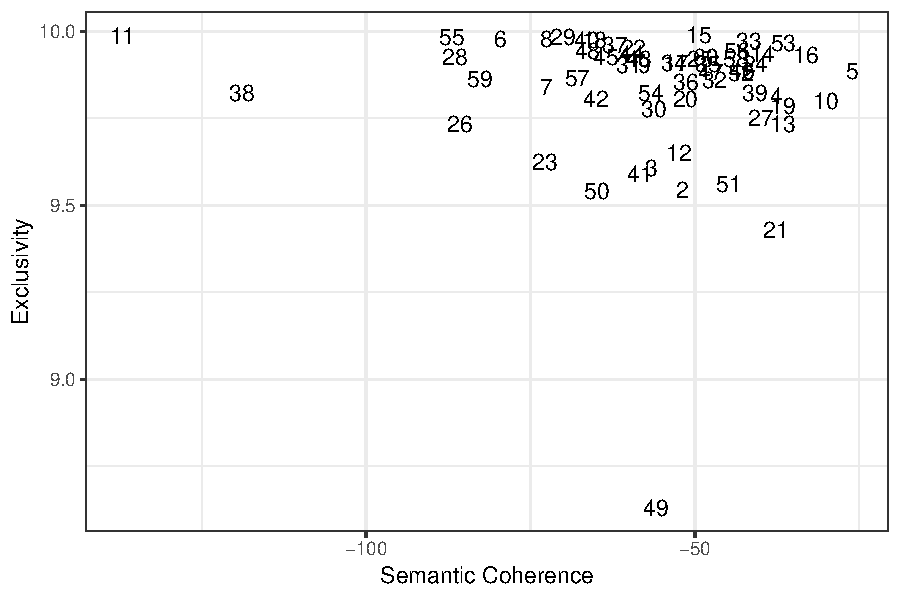
\includegraphics{figures/stm_60_coherence_exclusivity.pdf}
	\caption{Semantic coherence and exclusivity for each of the 60 topics in our main structural topic model. Coherence describes the extent to which the 10 top words in a topic model belong to the same underlying concept. Exclusivity measures whether the top words in one topic feature primarily in this topic, rather than being dispersed across a range of topics. The model performs well in this trade-off, as both coherence and exclusivity are high for most topics.}
	\label{fig:coherence_exclusivity}
\end{figure}




%% latex table generated in R 3.5.0 by xtable 1.8-2 package
% Wed Jul  4 14:14:10 2018
\begin{table}[ht]
\centering
\begin{tabular}{lrr}
  \hline
State & Democratic & Republican \\ 
  \hline
California &   9 &   6 \\ 
  Indiana &  46 &  54 \\ 
  Louisiana &  28 &  17 \\ 
  New York &  36 &  16 \\ 
  Texas &   2 &   7 \\ 
  Washington &  11 &   2 \\ 
   \hline
\end{tabular}
\caption{Descriptive statistics on the partisanship of the cities in the corpus.} 
\end{table}


%% latex table generated in R 3.4.3 by xtable 1.8-2 package
% Fri Mar  2 19:05:45 2018
\begin{table}[ht]
\centering
\begin{tabular}{lr}
  \hline
State & Cities \\ 
  \hline
Alabama &   1 \\ 
  Alaska &   1 \\ 
  Arizona &   6 \\ 
  California &  15 \\ 
  Colorado &   3 \\ 
  D.C. &   1 \\ 
  Florida &   6 \\ 
  Georgia &   1 \\ 
  Hawaii &   1 \\ 
  Idaho &   1 \\ 
  Illinois &   1 \\ 
  Indiana & 108 \\ 
  Kansas &   1 \\ 
  Kentucky &   2 \\ 
  Louisiana &  57 \\ 
  Maryland &   1 \\ 
  Massachusetts &   1 \\ 
  Michigan &   1 \\ 
  Minnesota &   2 \\ 
  Missouri &   2 \\ 
  Nebraska &   2 \\ 
  Nevada &   2 \\ 
  New Jersey &   2 \\ 
  New Mexico &   1 \\ 
  New York &  52 \\ 
  North Carolina &   4 \\ 
  Ohio &   4 \\ 
  Oklahoma &   2 \\ 
  Oregon &   1 \\ 
  Pennsylvania &   2 \\ 
  Tennessee &   2 \\ 
  Texas &  10 \\ 
  Virginia &   3 \\ 
  Washington &  13 \\ 
  Wisconsin &   2 \\ 
   \hline
\end{tabular}
\caption{Number of cities per state for which we have information about partisanship as well as the city's website URL.} 
\label{stateUrlSummary}
\end{table}



\bibliographystyle{chicago} % apsr stopped working for me
%\bibliographystyle{plainnat}
\bibliography{ref}


%\begin{figure}[htp]
  %  \centering
   % \caption{Five largest topic effects for the population covariate. The fact that the population and epidemiology topics are positively correlated with city size is indicative of the model's validity.}
    %  \label{stmEffectPop}
    % 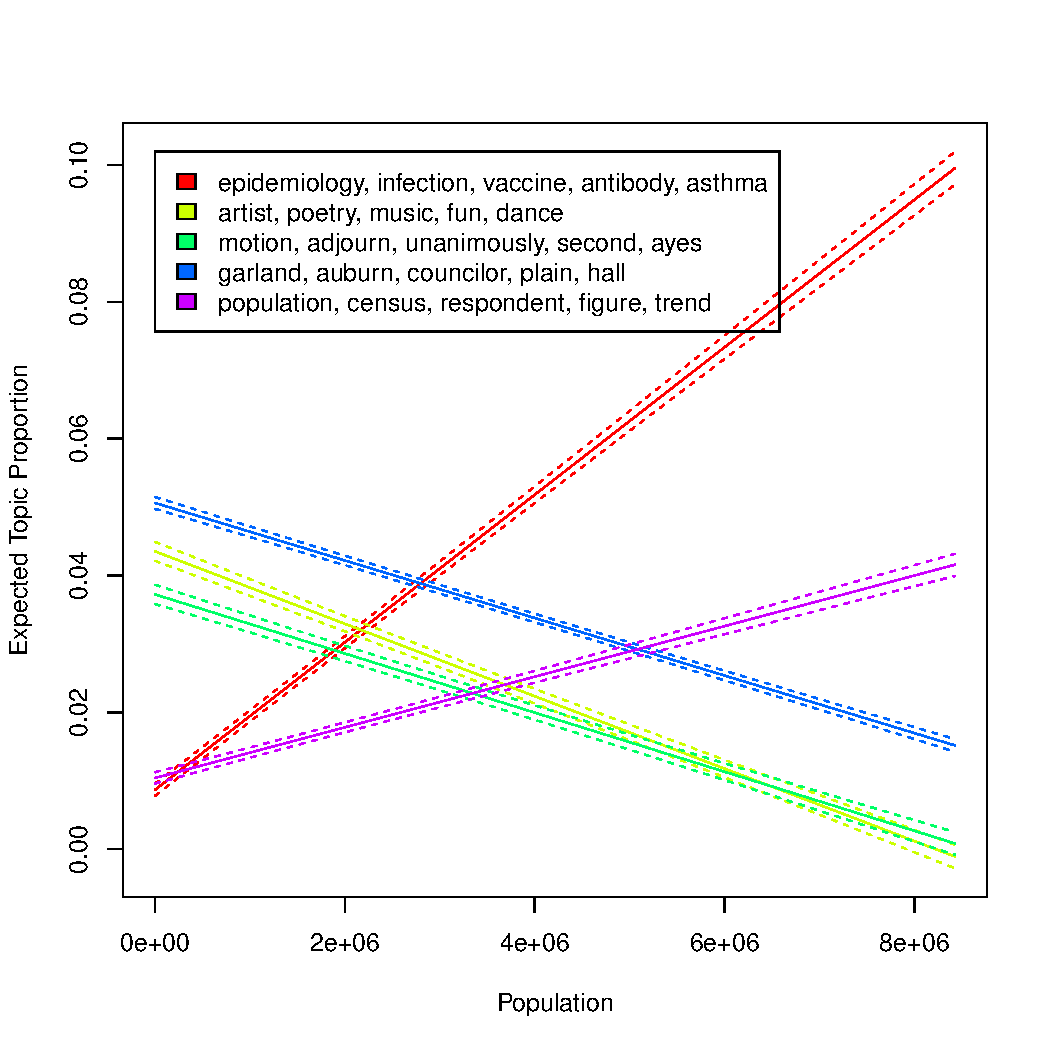
\includegraphics[width=\linewidth]{figures/stm_effect_pop.pdf}
% \end{figure}

% \begin{figure}[htp]
  %  \centering
   % \caption{Five largest topic effects for the median income covariate. The fact that the crime topic is most prevalent in poorer cities, good governance is the most positively correlated with income is indicative of the model's validity.}
   % \label{stmEffectIncome}
    %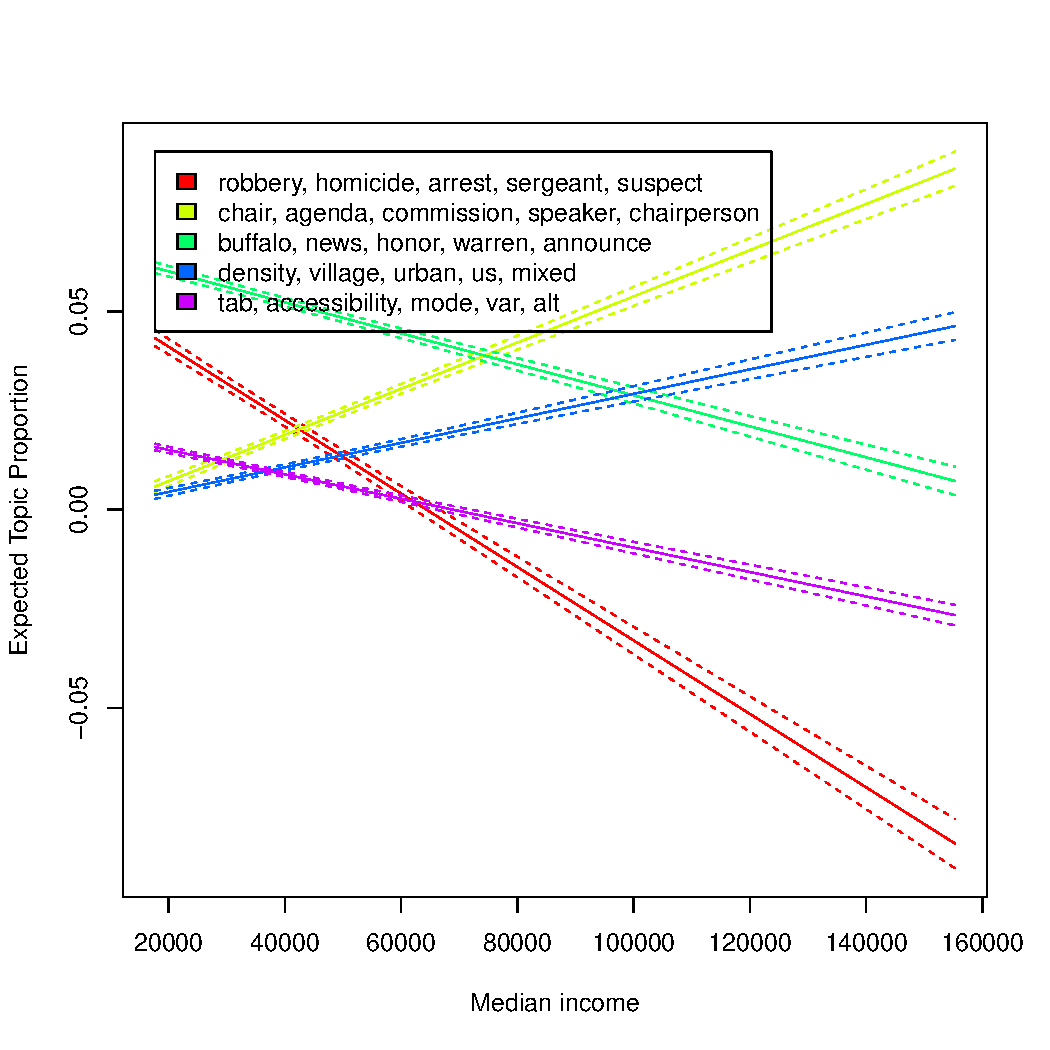
\includegraphics[width=\linewidth]{figures/stm_effect_income.pdf}
%\end{figure}


\end{document}





%\begin{enumerate}
%    \item Design
%    \begin{enumerate}
%        \item Choosing the sample
%        \item Finding URLs
%        \item list of .gov websites
%        \item Finding supporting data
%    \end{enumerate}
%    \item Scraping
%        \begin{enumerate}
%            \item wget
%            \item headless browser/Selenium
%            \item Beautifulsoup/rvest
%            \item APIs (httr)
%            \item Wayback Machine
%        \end{enumerate}
%    \item Pre-processing
%        \begin{enumerate}
%            \item Determining document filetype
%            \item File conversion
%            \item Conventional preprocessing (lowercase, numbers, punctuation)
%            \item Stemming and lemmatization
%            \item spellchecking
%            \item Dealing with duplicate text \& html documents in particular
%        \end{enumerate}
%    \item Analysis
%        \begin{enumerate}
%            \item LDA
%            \item Other topic models (structural, author, dynamic -- maybe?)
%            \item SVM (+ other machine learning classifiers?)
%            \item Fightin Words
%        \end{enumerate}
%\end{enumerate}
%
%
%
%
%
%
%% latex table generated in R 3.3.3 by xtable 1.8-2 package
%% Wed Mar 22 11:32:43 2017
%%\begin{table}[ht]
%%    \centering
%%    \begin{tabular}{lrrlrrl}
%%        \hline
%%        City & DemVotes & RepVotes & Winner & Change & Pop15 & url \\ 
%%        \hline
%%        Attica &  & 187 & Republican & 0 & 3117 & https://attica-in.gov/ \\ 
%%        Connersville & 1005 & 995 & Democratic & 1 & 13010 & http://connersvillecommunity.com/ \\ 
%%        Frankfort &  & 1748 & Republican & 0 & 16060 & http://frankfort-in.gov/ \\ 
%%        Huntingburg & 447 & 793 & Republican & 0 & 6035 & http://www.huntingburg-in.gov/ \\ 
%%        Indianapolis & 92830 & 56661 & Democratic & 1 & 862781 & http://www.indy.gov \\ 
%%        Lake Station & 1483 & 227 & Democratic & 0 & 12054 & http://www.lakestation-in.gov/ \\ 
%%        Linton & 785 & 692 & Democratic & 0 & 5284 & http://www.linton-in.gov/ \\ 
%%        Madison & 1192 & 1915 & Republican & 0 & 12040 & http://www.madison-in.gov/ \\ 
%%        Mitchell & 229 & 495 & Republican & 1 & 4252 & http://mitchell-in.com/ \\ 
%%        Monticello & 0 &  & Democratic & 0 & 5322 & http://www.monticelloin.gov/ \\ 
%%        North Vernon & 679 & 697 & Republican & 1 & 6619 & http://www.northvernon-in.gov/ \\ 
%%        Richmond & 3421 & 2731 & Democratic & 0 & 35854 & http://www.richmondindiana.gov/ \\ 
%%        Rockport & 286 & 272 & Democratic & 1 & 2223 & http://www.cityofrockport-in.gov/ \\ 
%%        South Bend & 8515 & 2074 & Democratic & 0 & 101516 & https://www.southbendin.gov/ \\ 
%%        Union City & 338 & 440 & Republican & 0 & 3447 & http://www.unioncity-in.gov/ \\ 
%%        Winchester & 606 & 524 & Democratic & 1 & 4769 & http://www.winchester-in.gov/ \\ 
%%        \hline
%%    \end{tabular}
%%    \caption{} 
%%\end{table}
%
%\subsection{Research Design}
%
%\begin{table}[ht]
%    \centering
%    \begin{tabular}{llr}
%        \hline
%        Variable & Unit & Source \\
%        \hline
%        Population size & 1000 people & Census \\
%        Population growth last 5 years & Percent & Census \\
%        Type of economy (agriculture/industry/services) & ? & Census \\
%        Economic performance (GDP?) & \$ & Census \\
%        Party of mayor before election & Rep/Dem/(Ind) & in.gov/sos/elections/ \\
%        Party of mayor after election & Rep/Dem/(Ind) & in.gov/sos/elections/ \\
%        Change of party control & 0/1 & in.gov/sos/elections/ \\
%        Presidential vote 2012 in county & Percent Rep & ? (but I have the data) \\
%        Unemployment rate & Percent & Census \\
%        Broadband speed & Avg. Mbps DL & broadbandmap.gov \\
%        \hline
%    \end{tabular}
%    \caption{List of covariates} 
%\end{table}
%
%
%
%\begin{enumerate}
%\item Corpus:
%\begin{enumerate}
%\item Last snapshots before the election (November 3, 2015 in Indiana; tbd. in Louisiana (probably February))
%\item First snapshot that is at least 2 months after the new government's inauguration (which is in January for Indiana, May for Louisiana)
%\end{enumerate}
%\item Preprocessing:
%\begin{enumerate}
%\item restrict corpus to:
%\begin{enumerate}
%\item documents belonging to cities in which a change of power occurred
%\item documents that were added, deleted or changed between the two snapshots
%\end{enumerate}
%\item words to lowercase
%\item remove punctuation
%\item stemming (Porter stemming algorithm?)
%\item Remove stop words (regular list of stop words is enough, since we use an asymmetric prior)
%\end{enumerate}
%\item Apply Grimmer's expressed agenda model to the corpus
%\begin{enumerate}
%\item Asymmetric prior
%\item Each document can have only one topic (in contrast to the author-topic model)
%\item Cities $i = 1,..., n = 15$
%\item Topic $k(k = 1,..., K )$
%\item Documents $j(j = 1,...,D_i)$ from city i
%\item Party covariate in the prior, where the deleted and unmodified documents are coded as from the first, and the added and modified documents from the second party
%\end{enumerate}
%\item Results
%\begin{enumerate}
%\item Label topics using Grimmer's automatic cluster labeling method, based on most commonly used words in documents belonging to topic
%\item Evaluate topics
%\end{enumerate}
%\end{enumerate}
%
%Validation:
%
%\begin{itemize}
%\item Do the above for cities in which no change of power occurred.
%\item Check whether there is higher than average turnover around the new year by comparing changes to non-election years (and also Louisiana, where elections are later).
%\item Check how long documents stay on websites on average. Use websites with a lot of snapshots for this (these exist for both small and large cities).
%\end{itemize}
%
%Problem with using this model: Grimmer's expressed agenda model uses Senators as the actors. Senators is also who he is substantively interested in. For us, the equivalent to Senators is cities. However, we care about parties, not cities.
%
%\subsection{Survival model}
%The existence of individual documents on municipal government websites can be though of as a survival process. No document stays on a website forever, and it appears to be a reasonable assumption that as documents get older and thus less relevant, they get replaced. The factors determining the steepness of the survival curve are the topic - fire safety regulations likely stay up longer than a bulletin on the annual spring banquet - and the change of party control after an election.
%
%\begin{quote}
%\textit{H1}: The older a document, the more likely it is to be removed.
%\end{quote}
%
%$S(t)$ has a downward slope. Admittedly, this is almost impossible not to be true. Also, test proportional, rising and falling hazard models.
%
%\begin{quote}
%\textit{H2}: Documents pertaining to administrative matters are less likely to be removed.
%\end{quote}
%
%Introduce a categorical variable for the top 10(?) topics. A negative coefficient for administrative topics would support this hypothesis.
%
%\begin{quote}
%\textit{H3}: Documents introduced by the opposing party are more likely to be removed.
%\end{quote}
%
%Introduce two variables into the survival model: One variable indicating which party has introduced a document, and a time-varying variable describing which party is currently in government. The hypothesis is tested through an interaction term between the two.
%
%\begin{quote}
%\textit{H4a}: Democrats are more likely to remove documents with topics pertaining to private enterprise, private schools.
%\end{quote}
%
%Interaction term between party in power and categorical topic variable.
%
%\begin{quote}
%\textit{H4b}: Republicans are more likely to remove documents with topics pertaining to social justice, equality, taxes, public schools, etc.
%\end{quote}
%
%Interaction term between party in power and categorical topic variable.
%
%\begin{quote}
%\textit{H5}: In line with their commitment to small government, Republicans are more likely than Democrats to remove documents.
%\end{quote}
%
%Party in power variable.\\
%
%
%This model will take up a lot of degrees of freedom. The rarity of snapshots for some cities might be a problem. Documents being changed and being removed can be modeled as competing risks.
%
%
%\begin{equation} 
%\label{eq1}
%\begin{split}
%Y & = \text{Party that introduced the document} \\
% & + \text{Party that is currently in power} \\
% & + \text{Topic 1, topic 2, ..., topic k} \\
% & + \text{Party that is currently in power} \times \text{Topic 1, topic 2, ..., topic k} \\
% & + \text{Days since start of mayoral term (control)}
%\end{split}
%\end{equation}
%
%
%
%
%
%After the counties, townships and cities that cannot be matched to the Census data\footnote{There are five cities that are not contained in the Census data} and duplicate websites (some cities have more than one website) are removed, 1813 domains/cities remain.
%
%These cities contain 90,616,865 people, and thus about 28\% of the U.S. population (see figure 1).
%
%\begin{figure}[htp]
%    \centering
%    \caption{Percentage of state population covered.}
%    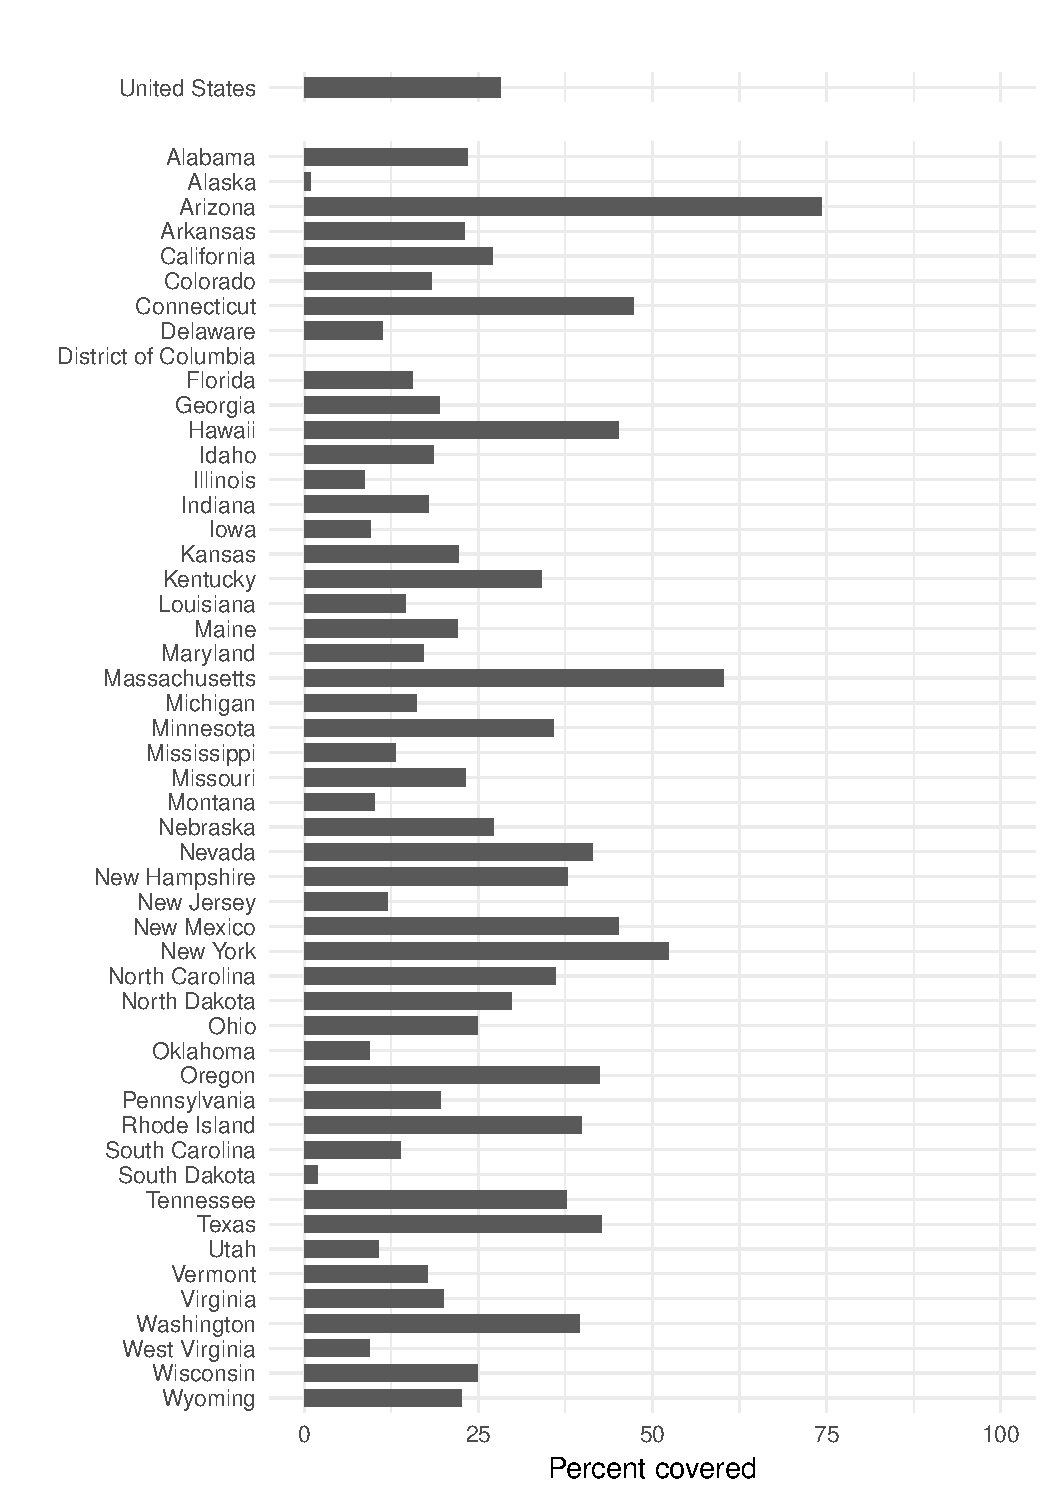
\includegraphics[width=0.9\linewidth,height=0.9\textheight]{figures/coverage_states.pdf}
%\end{figure}
%
%We use the resulting list of websites to acccess their copies stored in the Internet Archive's Wayback Machine. To this end, we rely on the Ruby Gem 'Wayback Machine Downloader'\footnote{https://github.com/hartator/wayback-machine-downloader} (WbMD). We supply the URL that each .gov website redirects to to the WbMD, which then downloads every file present in the WbM from a snapshot in October 2016, or, if not available, as soon as possible after this point.
%
%<Note: We have not actually done this last step for all websites (however, the R script which runs the Ruby package is already set up to do so once we need to). Instead 10 websites were randomly sampled from an older version of the GSA list, which still contained counties and townships, which is why one of the 10 websites is from Dutchess County, NY.>
%
%It would be fine to focus on Indiana as a case. First, we need to answer some preliminary questions about the data.
%
%\begin{enumerate}
%
%\item For what percentage and number of IN cities can we find data from the WBM?
%\item For how many election cycles can we find political leadership data for these matched cities?
%\item In what number and percentage of cities is the local leadership majority Republican? 
%\item Relatedly, in a typical election cycle, for how many cities do we see a transition in party leadership (i.e., a shift from majority D (R) to majority (R) D). 
%
%\end{enumerate}
%
%\begin{enumerate}
%    
%    \item 30 cities, with a combined population of 1,180,435. However, since only cities (as opposed to towns and villages) hold mayoral elections, only 16 of these, with a combined population of 1,094,383 can be matched to the election data.
%    \item 2015, 2011, 2007, 2003.
%    \item Of the 16 cities, 7 have Republican mayors after the 2015 elections.
%    \item In 6 cases, a shift of party control occurs, with 4 of these being Republican --> Democratic. 
%    
%\end{enumerate}
%
%
%
%
%\section{Running Application: Party Differences in Municipal Websites}
%
%
%\begin{landscape}
%\begin{table}[htbp]
%    %\caption{}
%    \begin{tabular}{|p{2cm}|c|p{3cm}|p{12cm}|l|}
%        \hline
%        Names & Year & Journal & Findings & Important? \\ \hline
%        Benedictis-Kessner, Justin De
%        Warshaw, Christopher & 2016 & JOP* & Regression discontinuity design. Democratic mayors spend more (but it is unclear on what, not the typical Democratic issue-areas), issue more debt, pay more interest & Yes \\ \hline
%        Caughey, Devin
%        Warshaw, Christopher
%        Xu, Yiqing & 2015 & Working Paper & Regression discontinuity design. Partisan composition of state governments affects state policy liberalism (composite index for the areas of social welfare, taxation, labor, civil rights, women’s rights, moral legislation, family planning, environment). & Somewhat \\ \hline
%        Einstein, Katherine Levine
%        Kogan, Vladimir & 2015 & Urban Affairs Review & Cities with more Democratic citizens spend more; more progressive (rather than regressive) forms of taxation; pursue intergov. aid more; spend more on police, fire, parks \& recreation & Somewhat \\ \hline
%        Einstein, Katherine Levine
%        Glick, David M. & 2015 & Working Paper & Survey of 72 mayors. Unlike Republican mayors, roughly half of Democrats seem to agree that cities should aim to reduce inequality. Democratic mayors also seem to favor redistribution to accomplish that goal. & Somewhat \\ \hline
%        Kiewiet, D Roderick
%        Mccubbins, Mathew D & 2014 & Annual Review & City budgets have been severeley constrained since the Great Recession. Spending has thus decreased in general. Lack of funds means that there is not much discretion for partisanship. & Somewhat \\ \hline
%        Tausanovitch, Chris
%        Warshaw, Christopher & 2014 & APSR* & Cities are responsive (taxes, expenditures, regressiveness of taxation) to citizens' conservatism/liberalism. Partisan elections do not make cities more or less responsive. & Yes \\ \hline
%        Guillamón, Ma Dolores
%        Bastida, Francisco
%        Benito, Bernardino & 2013 & European Journal of Law and Economics & Police spending in Spain. Conservative parties spend more on police. Spending is higher before elections. Also contains a useful overview of the literature. & Yes \\ \hline
%    \end{tabular}
%    \label{}
%\end{table}
%\end{landscape}
%
%\begin{landscape}
%    \begin{table}[htbp]
%        %\caption{}
%        \begin{tabular}{|p{2cm}|c|p{3cm}|p{12cm}|l|}
%            \hline
%            Names & Year & Journal & Findings & Important? \\ \hline
%            Gerber, Elisabeth R. & 2013 & Cityscape & Partisanship of both citizens and elected city officials separately affect climate policy. & Yes \\ \hline
%            Solé-Ollé, Albert
%            Viladecans-Marsal, Elisabet & 2013 & Journal of Urban Economics & Spanish cities. The authors "employ a regression discontinuity design to document that cities controlled by left-wing parties convert much less land from rural to urban uses than is the case in similar cities con- trolled by the right". Partisanship might also affect housing construction and price growth. & Yes \\ \hline
%            Gerber, Elisabeth R.
%            Hopkins, Daniel J. & 2011 & AJPS & Regression discontinuity design. Democratic mayors spend less on public safety. All other policy areas (including taxation) are unaffected. & Yes \\ \hline
%            Trounstine, Jessica & 2010 & Annual Review & Race and ethnicity in local elections (not relevant to us). Partisan elections have higher turnout; non-partisan elections still tend to have some partisanship in them because voters learn about party of candidates from media. Non-partisan elections favor Republicans/upper class. Mixed evidence for whether partisanship of mayor is important for policy. & Somewhat \\ \hline
%            Palus, Christine Kelleher & 2010 & State and Local Government Review & Ideology (liberal/conservative) of citizen is well represented by gov. spending in five areas: (1) community development, housing, and conservation, (2) health and human services, (3) culture, the arts, and recreation, (4) environmental programs, and (5) transportation. & Somewhat \\ \hline
%            Ferreira, Fernando
%            Gyourko, Joseph & 2009 & The Quarterly Journal of Economics & Regression discontinuity design. Null results for spending and city gov. size with regard to mayor partisanship. & Yes \\ \hline
%            Ansolabehere, Stephen
%            Snyder, James M. & 2006 & Scandinavian Journal of Economics & Despite the journal, this is about the U.S. The important finding (for us) is the fact that counties whose government is controlled by the same party as the state government, receive more funding (county's share of state transfers, normalized by county pop.) from the state. & Somewhat \\ \hline
%            Murphy, Russell D. & 2002 & Annual Review & Not useful. Too philosophical; mostly cites papers written a hundred years ago. Also exclusively about larger cities. & No \\ \hline
%        \end{tabular}
%        \label{}
%    \end{table}
%\end{landscape}
%
%\begin{landscape}
%    \begin{table}[htbp]
%        %\caption{}
%        \begin{tabular}{|p{2cm}|c|p{3cm}|p{12cm}|l|}
%            \hline
%            Names & Year & Journal & Findings & Important? \\ \hline
%            Armstrong, Cory L. & 2011 & Government Information Quarterly & Comparison of county and school board websites in Florida (where the two align) with regard to transparency (presence or absence of public records). Manual content analysis (undergrads told to look around for 15 minutes). School board websites, more professional websites, and websites in Republican-dominated counties are found to be more transparent. & Yes \\ \hline
%            Cegarra-Navarro, Juan
%            Pachón, José
%            Cegarra, José & 2012 & International Journal of Information Management & Survey of Spanish municipal government officials (specifically, the city website managers). Respondents are asked about the features of their websites, the level of civic engagement and the size of their municipality. More sophisticated websites are correlated with greater civic engagement and greater use of e-government functions. & Yes \\ \hline
%            Dolson, Jordan
%            Young, Robert & 2012 & Canadian Journal of Urban Research & Determinants of website content. Three categories: e-content (city information on website), e-participation, social media use. Tables on page 15 show frequencies of these categories across sites, and might be useful to inform our topics. Larger cities have better websites. Population growth and immigration are also tested, but the findings are somewhat inconclusive. & Yes \\ \hline
%            Feeney, Mary K.
%            Brown, Adrian & 2017 & Government Information Quarterly & 500 U.S. city websites at two points in time (2010-2014). Count model of website features regarding information, e-services, utilities, transparency and civic engagement. Having a larger population leads to more features. Relying on a website contractor leads to more information and transparency. The authors say that mayor-councils are negatively correlated with website sophistication, but their regression tables state the opposite. & Yes \\ \hline
%            Kaylor, Charles
%            Deshazo, Randy
%            Van Eck, David & 2001 & Government Information Quarterly & Model of best practices of e-government. Table 1 lists a number of possible ways this manifests, could be useful for our theory. & Somewhat \\ \hline
%            Ansolabehere, Stephen
%            Urban, Florian & 2002 & Cities & Websites of 20 major cities across the world. Is website content correlated with city characteristics? Not particularly systematic, and the findings are inconclusive. & Somewhat \\ \hline
%            Jeffres, Leo W.
%            Lin, Carolyn A. & 2006 & Journal of Computer-Mediated Communication & 50 largest metropolitan areas in the U.S. Features include information about city, opportunities for citizen feedback, galleries of photos, links, etc.  Purely descriptive analysis, doesn't contain anything that isn't covered in any of the other aricles. & No \\ \hline
%        \end{tabular}
%        \label{}
%    \end{table}
%\end{landscape}
%
%\subsection{Informative Dirichlet model}
%%However, \cite{Monroe2008} advise against using these types of methods in this context because they get the data generation process backwards: Our theory assumes that party leads to variation in writing, and yet we rely on the documents to predict party, in spite of the fact that we actually have perfect knowledge of it.
%
%For the analysis of the data, we present two approaches, the first being the informative dirichlet model developed by \citep{Monroe2008}. This approach aims to account for the fact that some words naturally occur more than others by applying a Dirichlet prior based on the distribution of words in random text. Table \ref{tabFightinIN} shows the top words for both Democrats and Republicans - and accomplishes, to some extent, the goal of \citep{Monroe2008} of banishing frequent words from this list and supplanting them with text with greater semantic, and in our case, partisan meaning. 
%
%In Indiana, Democrats exhibit a preference for words related to public finance, such as 'fund', 'budget', or 'tax', indicative of a greater willingness to emphasize the city's efforts to raise and spend money. This finding is consistent with \citep{Einstein2015}, who show that Democratic mayors tend to favor greater spending. Beyond the focus on public finance, the words preferably used by Democrats do not fall into any particularly congruent categories, and largely sort into various areas related to city administration - i.e. `council', `services', `budget', `committee', `contract', etc. If there is theme around the words preferred by Republicans, it seems to center around city planning - street, fire, water, building, construction, park. These words suggest that the hands-off approach favored by Republicans results in a focus on supporting infrastructure and logistics.
%
%%Partisan top words - fightin words Indiana
%% latex table generated in R 3.4.1 by xtable 1.8-2 package
% Fri Oct 20 10:49:17 2017
\begin{table}[ht]
\centering
\begingroup\fontsize{9pt}{10pt}\selectfont
\begin{tabular}{lrlr}
  \hline
Word (D) & z-Score (D) & Word (R) & z-Score (R) \\ 
  \hline
said & 86.20 & request & 69.41 \\ 
  proposal & 70.98 & member & 67.45 \\ 
  fund & 59.22 & street & 47.84 \\ 
  county & 54.15 & motion & 46.35 \\ 
  asked & 52.62 & councilor & 45.69 \\ 
  budget & 49.40 & main & 44.34 \\ 
  stated & 46.90 & goods & 44.33 \\ 
  tax & 41.79 & use & 43.43 \\ 
  fort & 41.17 & tree & 42.77 \\ 
  ms & 40.76 & amp & 42.48 \\ 
  division & 38.01 & water & 41.45 \\ 
  million & 36.62 & downtown & 40.66 \\ 
  grants & 35.21 & pm & 39.60 \\ 
  introduced & 34.85 & sign & 39.28 \\ 
  contract & 34.36 & st & 38.23 \\ 
  revenue & 34.33 & plan & 38.20 \\ 
  general & 34.17 & rd & 37.71 \\ 
  chair & 32.01 & site & 37.19 \\ 
  brown & 31.86 & docket & 37.03 \\ 
  federal & 31.46 & trees & 36.56 \\ 
  metropolitan & 31.25 & plat & 36.15 \\ 
  management & 30.69 & old & 35.44 \\ 
  agency & 30.35 & residential & 34.65 \\ 
  approves & 29.66 & area & 34.31 \\ 
  authorizes & 29.11 & variance & 33.50 \\ 
  technology & 28.45 & th & 33.20 \\ 
  provide & 27.43 & utility & 33.11 \\ 
  dollars & 27.30 & ordinance & 32.04 \\ 
  consolidated & 26.29 & carter & 31.40 \\ 
  justice & 25.93 & approve & 31.40 \\ 
  parks & 25.79 & building & 30.78 \\ 
  lewis & 25.73 & feet & 30.16 \\ 
  increase & 25.66 & news & 29.37 \\ 
  digest & 25.60 & city & 29.26 \\ 
  support & 25.43 & lots & 29.19 \\ 
  oliver & 25.43 & lot & 28.89 \\ 
  animal & 25.02 & aid & 28.54 \\ 
  gray & 24.72 & overlay & 28.53 \\ 
  capital & 24.54 & home & 28.52 \\ 
  services & 24.53 & democrat & 28.40 \\ 
  amends & 23.84 & republican & 28.25 \\ 
  criminal & 23.70 & uses & 28.05 \\ 
  enterprise & 23.62 & must & 27.57 \\ 
  mayors & 23.51 & legal & 26.64 \\ 
  court & 22.90 & zoning & 26.53 \\ 
  township & 22.86 & councilors & 26.50 \\ 
  controls & 22.54 & river & 26.48 \\ 
  funded & 22.28 & stellar & 26.40 \\ 
  referred & 22.16 & common & 26.15 \\ 
  fiscal & 22.10 & rep & 26.03 \\ 
   \hline
\end{tabular}
\endgroup
\caption{Top 50 democratic and Republican words (Indiana), according to the informed 
             Dirichlet model of Monroe et al. (2008).} 
\label{tabFightinIN}
\end{table}

 %\ref{tabFightinIN}
%
%For Lousiana, the results (see table \ref{tabFightinLA}) are less coherent. Only one of the finance-related terms appears again for Democrats - specifically `fund', although `rate' might also be used in a financial context. Beyond that, some focus on a `historic' `'district of a city seems evident, as is the use of some words - `infrastructure', `water', `building' that were used for Republicans in Indiana. Conversely, Republicans are now missing these words, and their preferred terms generally do not seem to follow any particular theme.
%
%%Partisan top words - fightin words Louisiana
%% latex table generated in R 3.4.3 by xtable 1.8-2 package
% Tue Dec 26 15:00:39 2017
\begin{table}[ht]
\centering
\begingroup\fontsize{9pt}{10pt}\selectfont
\begin{tabular}{lrlr}
  \hline
Word (D) & z-Score (D) & Word (R) & z-Score (R) \\ 
  \hline
otherwise & 20.73 & say & 86.18 \\ 
  health & 18.65 & ordinance & 77.67 \\ 
  respect & 17.98 & summary & 59.81 \\ 
  use & 16.62 & bid & 58.98 \\ 
  officer & 16.22 & council & 46.92 \\ 
  staff & 15.87 & amount & 41.21 \\ 
  district & 15.82 & official & 39.79 \\ 
  historic & 15.51 & mayor & 39.07 \\ 
  datum & 15.19 & accordance & 37.91 \\ 
  fund & 15.02 & boulevard & 37.78 \\ 
  thereto & 14.86 & weekend & 35.41 \\ 
  building & 14.70 & weather & 34.34 \\ 
  street & 14.69 & seal & 33.27 \\ 
  total & 14.60 & responsive & 33.15 \\ 
  window & 14.50 & veteran & 31.96 \\ 
  applicant & 14.41 & resolution & 29.52 \\ 
  exist & 14.19 & hold & 28.71 \\ 
  housing & 14.13 & gathering & 28.32 \\ 
  provide & 13.84 & furnish & 27.36 \\ 
  review & 13.58 & councilman & 27.19 \\ 
  source & 13.54 & meeting & 26.74 \\ 
  neighborhood & 13.09 & exceed & 26.54 \\ 
  revenue & 12.99 & show & 26.44 \\ 
  target & 12.88 & emergency & 26.01 \\ 
  policy & 12.75 & resident & 25.23 \\ 
  training & 12.52 & city & 24.89 \\ 
  process & 12.51 & accept & 24.73 \\ 
  actual & 12.45 & visit & 24.67 \\ 
  population & 12.04 & wheeler & 24.21 \\ 
  green & 11.95 & night & 24.11 \\ 
  rate & 11.70 & purchase & 24.00 \\ 
  infrastructure & 11.68 & theater & 23.76 \\ 
  urban & 11.46 & parish & 23.63 \\ 
  average & 11.45 & sweep & 23.39 \\ 
  retention & 11.22 & inc & 23.27 \\ 
  master & 11.03 & tonight & 22.09 \\ 
  bureau & 10.93 & recreation & 21.92 \\ 
  roof & 10.90 & mike & 21.82 \\ 
  strategy & 10.89 & park & 21.78 \\ 
  water & 10.82 & department & 21.71 \\ 
  construct & 10.79 & movie & 21.65 \\ 
  residence & 10.57 & tropical & 21.50 \\ 
  reduce & 10.47 & hall & 21.49 \\ 
  relative & 10.46 & contract & 21.31 \\ 
  construction & 10.46 & pet & 21.24 \\ 
  monthly & 10.46 & morning & 21.08 \\ 
  chapter & 10.43 & begin & 20.84 \\ 
  individual & 10.35 & information & 20.78 \\ 
  design & 10.29 & beach & 20.60 \\ 
  standard & 10.24 & approve & 20.56 \\ 
   \hline
\end{tabular}
\endgroup
\caption{Top 50 Democratic and Republican words (Louisiana), according to the informed Dirichlet model of Monroe et al. (2008).} 
\label{tabFightinLA}
\end{table}

 %\ref{tabFightinLA}
%
%The weakness of the fightin' words method is evident here, as a list of words does not necessarily provide sufficient information to glean preferred topics from. This is especially the case when the texts are spread across a broad number of issue-areas, with little semantic similarity. In \citep{Monroe2008}, the authors focus on the fairly constrained corpus of U.S. Senate speeches with respect to abortion - our context, by comparison, is far more eclectic.








